%%%%%%%%%%%%%%%%%%%%%%%%%%%%%%%%%%%%%%%%%%%%%%%%%%%%%%%%%%%%%%%%%%%%%
%%                                                                 %%
%% Please do not use \input{...} to include other tex files.       %%
%% Submit your LaTeX manuscript as one .tex document.              %%
%%                                                                 %%
%%%%%%%%%%%%%%%%%%%%%%%%%%%%%%%%%%%%%%%%%%%%%%%%%%%%%%%%%%%%%%%%%%%%%

\documentclass[pdflatex,mathphys]{jnl}

\usepackage{caption}
\usepackage{graphicx}
\usepackage{subcaption}
\captionsetup{justification=justified, font=small}

% Removing the resetlabels option ensures that the numbering continues from the
% main bibliography to the methods bibliography.
\usepackage[]{multibib}
\newcites{Meth}{Methods References}
\newcites{Supp}{Supplementary References}

\usepackage{paralist}

\usepackage{siunitx}

\raggedbottom

% ============================================================================
% FIGURE STRUCTURE (driven by the BoG 2026 talk deck + transcript):
%   Fig 1  Genome-wide subtelomeric homology + PHR extent        (deck slides 3,4)
%   Fig 2  Pangenome similarity structure + communities          (deck slides 6,10,12)
%   Fig 3  Architecture of representative communities (browser)  (deck slides 14,15,16)
%   Fig 4  Sequence similarity predicts 3D proximity             (deck slides 20,21,22)
%   Fig 5  Pedigree-resolved subtelomeric exchange (untangle)    (deck slides 24,26)
% Per author direction Extended Data is a single figure: ED1 = mouse meiotic
% Hi-C (deck slide 20). The other analyses remain in the body/methods text.
% ASSET NOTE: Fig1-5 currently embed slide-derived PNGs as faithful placeholders.
% Publication-quality vector versions must be regenerated from paper_prep/figures/.
% ============================================================================

\begin{document}

\title[Concerted evolution of human subtelomeres]{Concerted evolution and unorthodox recombination of human subtelomeres}

\author*[1]{\fnm{Andrea} \sur{Guarracino}}\email{aguarracino@tgen.org}
\author[2]{\fnm{Angela} \sur{Gyamfi}}
\author*[3]{\fnm{Erik} \sur{Garrison}}\email{egarris5@uthsc.edu}

\affil[1]{Bioinnovation and Genome Sciences, The Translational Genomics Research Institute (TGen), Phoenix, AZ 85004, USA}
\affil[2]{St. Jude Children's Research Hospital, Memphis, TN 38105, USA}
\affil[3]{Department of Genetics, Genomics and Informatics, University of Tennessee Health Science Center, 71 S Manassas St, Memphis, 38163, Tennessee, USA}

\abstract{
Human subtelomeric regions are among the most dynamic and structurally complex parts of our genome, yet their interchromosomal relationships have remained difficult to characterize due to the limitations of both assembly completeness and alignment methodology. Here we present the most comprehensive survey of subtelomeric sequence relationships to date, leveraging 466 near-complete haplotype assemblies from the Human Pangenome Reference Consortium (HPRC) version 2. To analyze these regions, we introduce the implicit pangenome graph, a reference-free alignment approach that performs all-to-all pairwise comparisons across haplotypes, sampling approximately 12\% of all possible combinations, without imposing chromosomal partitioning or positional bias. This yields a truly unbiased view of interchromosomal homology across the pangenome, where every haplotype serves as its own point of reference, allowing a systematic and universal view of human subtelomeric evolution. A genome-wide survey of alignment identity reveals extended regions of interchromosomal homology spanning tens to hundreds of kilobases at nearly all subtelomeres, comparable in scale to canonical pseudohomologous systems such as PAR2 on the sex chromosomes. This dramatically expands the scope of known pseudohomologous regions in the human genome to include almost all subtelomeric regions. Cladistic analysis based on neighbor-joining trees of subtelomeric similarity uncovers both expected relationships (Xp/Yp and Xq/Yq via the pseudoautosomal regions, acrocentric short arms) and novel associations, including strong 10p--18p homology, a tightly linked clade involving 22q, 21q, 19q, 1q, 13q, and 17q, and extended DUX4-containing homology between 4q and 10q with wide copy number diversity. A large clade of many chromosome arms shares homology at moderate similarity, suggesting broad ongoing interchromosomal exchange. Principal component and community detection analyses of the similarity matrix further resolve subtelomeric clustering across human populations. We hypothesized that these patterns are maintained by recombination facilitated by the physical proximity of subtelomeres at the nuclear envelope, and tested this across orthogonal three-dimensional genome maps. Bulk Hi-C, Pore-C, and CiFi, single-cell Dip-C and sperm scHi-C, and mouse meiotic Hi-C all show that chromosome arms sharing a sequence-defined community make significantly more interchromosomal contact at their subtelomeres than arms in different communities, across all eight human contact datasets ($p<0.01$), and that sequence similarity predicts nuclear proximity (Mantel $\rho$ up to 0.85), a relationship that strengthens rather than weakens when acrocentric and sex chromosomes are excluded. This correlation peaks in mouse meiosis at the zygotene stage (Mantel $\rho=0.718$), when the telomere bouquet clusters chromosome ends against the nuclear envelope. Finally, a three-generation telomere-to-telomere pedigree captures the recombination directly: of 538 interchromosomal patches transmitted between generations, 494 (92\%) fall within the same sequence-similarity communities, including ectopic gene-conversion tracts at perfect identity and crossover-like breakpoints. Our work exposes the extent to which ongoing recombination, organized by the three-dimensional architecture of the nucleus, shapes these highly dynamic and poorly understood regions of the genome.
}

\keywords{pangenome, subtelomere, pseudohomologous region, concerted evolution, recombination, Hi-C, meiotic bouquet, HPRC v2}

\maketitle

The chromosome ends of the human genome were the first regions in which
inter-chromosomal sequence exchange, an unorthodox recombination class that
operates between non-homologous chromosomes, was identified
\cite{Brown1990,Wilkie1991,Trask1991}.
PAR1 and PAR2 sustain obligate meiotic crossover between the sex chromosomes
\cite{Rouyer1986,sexchrompars_bellott2024}; the acrocentric rDNA-bearing short
arms 13p, 14p, 15p, 21p and 22p share blocks of identity that recombine in
pre-meiotic nucleoli \cite{acrocentric_Altemose2022,acrocentric_Guarracino2025ape};
the D4Z4 macrosatellite on 4q35 and 10q26 underlies FSHD
\cite{dux4_d4z4_fshd_lemmers2010worldwide}, with degenerate D4Z4-like copies
on at least ten additional chromosomes revealed by T2T-CHM13 \cite{Salsi2026fshd},
and is reactivated as an oncofetal programme in diverse solid cancers
\cite{dux4_cancer_Chew2019}.
Cytogenetic FISH and BAC-walking mapped multi-chromosomal duplicons across
roughly half of the 48 arms
\cite{Mefford2001,MeffordTrask2002,Linardopoulou2005,Riethman2004,Ambrosini2007};
that body of work established the cytogenetic reality but surveyed only a slice
of the available inter-chromosomal homology, because no reference assembly was
complete to the telomeres \cite{Nurk2022} and per-chromosome alignment frames
hid trans-chromosomal sharing.
Earlier pangenome builds, including HPRCv1, assembled chromosomes independently
for technical reasons, which masked trans-chromosomal sharing in the graph
itself \cite{Liao2023}.
The HPRC v2 release delivers near-T2T haplotype-resolved assemblies for 233
individuals from five superpopulations \cite{hprc_hprcv2_2025}, removing both
constraints.
We revisit subtelomeric architecture without chromosomal partitioning, studying
for the first time at population scale the evolution of complete chromosome
ends in humans, and ask how extensive inter-chromosomal sharing is, whether it
predicts three-dimensional nuclear proximity, and whether the events that build
the population structure can be observed directly in pedigrees.

We treat every haplotype as its own reference.
From the 233 individuals we used 465 HPRC v2 haplotype assemblies plus
CHM13v2.0 (Methods), extracted 18,827 telomere-anchored 500 kb flanks across
48 chromosome arms and ran
wfmash all-vs-all at 95\% minimum identity \cite{Guarracino2023} without
restricting alignment to homologous chromosomes.
The resulting PAF set is the implicit pangenome graph: nodes are flanks, edges
are wfmash alignments, and the canonical query is the IMPG transitive closure
\cite{pangenome_graphs_impg_GarrisonGuarracino2023,pangenome_graphs_impg_IMPG2023}.
The full pairwise space across haplotypes is on the order of $10^{24}$
base-pair comparisons and is intractable at genome scale; even restricted to
18,827 flanks the $C(18827, 2) = 177$ million pairs are intractable at
single-assembly resolution.
In a panmictic population most pairwise alignments are redundant, and wfmash
k-mer prefiltering evaluates 11.6\% (12\% rounded) of pairs.
This sampling rate sits $230\times$ above the Erd\H{o}s and R\'{e}nyi
connectivity threshold $p^{*} = \log(n)/n = 5.2 \times 10^{-4}$ for
$n = 18827$, so transitive closure recovers virtually every subtelomere in the
dataset (Methods).
We define a pseudohomologous region (PHR) as a flank window in which IMPG
transitive closure recovers alignment to $\geq 5$ segments on $\geq 2$
different chromosomes at identity $\geq 95\%$, total aligned length $\geq 3$
kb \cite{Garrison2024pggb}.
This filter yields 15,668 PHRs (83.2\% of flanks) on 41 of 48 arms; the 7
remaining arms (chr2\_p, chr3\_p, chr5\_p, chr8\_q, chr11\_q, chr14\_q,
chr18\_q) carry no detectable inter-chromosomal homology and provide the
silent-arm $S_{\mathrm{all}}$ negative control.

The genome-wide survey reveals telomere-anchored high-identity blocks at nearly
every chromosome end (Fig.~\ref{fig:fig1}a).
Each chromosome is rendered in 100 kb windows coloured by the number of
distinct partner chromosomes a window aligns to elsewhere in the pangenome,
together with a region track (centromere, PAR, PHR, terminal repeat), making
both the identity and the depth of inter-chromosomal sharing visible in one
view.
Detected PHRs span tens to hundreds of kilobases (Fig.~\ref{fig:fig1}b; median
105 kb, mean 144 kb, range 5 kb to 500 kb), with the upper bound determined by
the 500 kb flank window rather than by biology.
Excluding the acrocentric short arms and PAR1/PAR2, the non-acrocentric,
non-PAR PHRs total 3.510 Mb of subtelomeric pangenome sequence.
The median PHR is 31\% of the length of PAR2 (334 kb), and the mean PHR is
43\% of PAR2.
The largest fully homogenised inter-chromosomal region known in the human
genome \cite{sexchrompars_bellott2024} is now flanked, at population scale, by
15,668 examples of structurally comparable architecture, though PAR2 is fully
homogenised by obligate crossover and most other PHRs are not.

Read directly, the 15,668-sequence implicit graph forms a single connected
component (Fig.~\ref{fig:fig2}a, PGGB/odgi layout) that is too tangled to
interpret node by node; we therefore reduce it to arm-level and sequence-level
Jaccard matrices as the analytical substrate (Methods).
The 41 signal-bearing arms partition into 15 communities at the arm level
(Fig.~\ref{fig:fig2}c) and 50 communities at the sequence level (modularity 0.97; Methods).
The similarity matrix is not a uniform gradient: it has discrete cladal
structure, with groups of arms that share sequence and gaps between them
(Fig.~\ref{fig:fig2}b).
A neighbour-joining tree built on the $41 \times 41$ arm-level Jaccard
distance matrix recovers six well-supported groupings that match every known
case of inter-chromosomal subtelomere homology (Fig.~\ref{fig:fig2}b shows the
same matrix as a heatmap with UPGMA dendrogram).
We use `clade' as an ordering device for the NJ tree, not as an evolutionary
claim; the tree groups arms by Jaccard similarity and we do not propose a
phylogenetic relationship between subtelomeric ends.
PAR1 (Xp, Yp) and PAR2 (Xq, Yq) form two groupings
\cite{sexchrompars_acquaviva2020}.
The acrocentric short arms 13p, 14p, 15p, 21p and 22p form a third grouping
consistent with their shared rDNA arrays \cite{acrocentric_Altemose2022}.
A 10p/18p grouping reproduces the high-identity pair first reported by
Linardopoulou and colleagues \cite{Linardopoulou2005}, anchored by tubulin
gene arrays on 10p and a single-copy counterpart on 18p.
A tight q-arm grouping comprising 22q, 21q, 19q, 1q, 13q and 17q is, to our
knowledge, the first cladistic recovery of this composite group at population
scale.
Finally, 4q and 10q pair through the D4Z4 macrosatellite
\cite{dux4_d4z4_fshd_lemmers2010worldwide,Cabianca2012}, with wide copy-number
diversity across the 465 haplotypes (DUX4 family copy counts range 0 to 22).
Placement of each grouping is robust to algorithm choice: Leiden on a
kernel-weighted version of the same distance matrix yields 15 arm-level
communities (mean silhouette 0.347, $k = 15$), and the six groupings map
one-to-one to C15 (PAR1), C14 (PAR2), C7 (acrocentric p-arms), C2 (10p/18p),
C6 (\{22q, 21q, 19q, 1q, 13q, 17q\}) and C1 (4q/10q DUX4).
UPGMA at $k = 14$ agrees with Leiden on 12 of 15 communities.
A 1,000-replicate character-level bootstrap recovers PAR1, PAR2 and 10p/18p at
100\%, 4q/10q DUX4 at 99.4\% and the acrocentric p-arms at 52\% NJ / 87\%
UPGMA; the 6-arm tight q-arm grouping collapses to 0.1\% under the
chromosome-granular per-PHR surrogate, a data-granularity artefact (Methods).
Deeper internal edges have 32--90\% support, mirroring the well-known fact that
subtelomere-internal duplicon order is not strictly nested at the chromosome
level \cite{Skaletsky2003,Rudd2009}.

To make the communities concrete we examine three at the sequence level, so a
reader need not return to a genome browser (Fig.~\ref{fig:fig3}).
Community C1 (4q/10q; Fig.~\ref{fig:fig3}a) is the D4Z4/DUX4 system: the 4q35
and 10q26 ends carry homologous DUX4L macrosatellite arrays, FRG1/FRG2 paralog
families and shared segmental duplications, with copy number ranging from 0 to
22 across the 465 haplotypes
\cite{dux4_d4z4_fshd_lemmers2010worldwide,Cabianca2012}.
Community C2 (10p/18p; Fig.~\ref{fig:fig3}b) is anchored by the TUBB8B tubulin
gene array, present in tandem copies on 10p and as a single-copy counterpart on
18p, reproducing the high-identity pair of Linardopoulou and colleagues
\cite{Linardopoulou2005}.
Community C11 (5q/6q; Fig.~\ref{fig:fig3}c) is built on the OR4F
olfactory-receptor family and its pseudogenes, representative of the
olfactory-receptor and hub-pseudogene content that recurs across the q-arm
communities.
Each community thus carries a duplicon-anchor signature (D4Z4/DUX4 in 4q/10q;
tubulins in 10p/18p; rDNA in the acrocentrics; olfactory-receptor and
hub-pseudogene families in the q-arm grouping).

Beyond these anchors, the 15 arm-level communities are internally heterogeneous
rather than monolithic.
On the joint axes of cross-arm sequence rate and per-community silhouette the
41 arms split 4/28/9 into homogeneous, polymorphic and fully interchangeable
classes, refining the qualitative 8/34/7
architectural skeleton from FISH-era inspection
\cite{Linardopoulou2005,Stong2014}.
Across 5,946 paired distances from the nine multi-arm communities,
within-haplotype-pair allelic distance is shorter than cross-paralog distance
in 8 of 9 communities (combined $p < 10^{-300}$); the exception is the rDNA-bearing acrocentric p-arms
(C7), homogenised more deeply than within-individual variation
\cite{acrocentric_Altemose2022}.
In 39 of 48 arms the number of distinct chromosome contributors per flank
window decreases monotonically with distance from the telomere, and in 39 of
41 signal-bearing arms a single-breakpoint piecewise model outperforms a
linear model, generalising the two-domain
Flint--Mefford model of a proximal unique segment and a distal duplicon-rich
segment to the pangenome \cite{Flint1997,MeffordTrask2002}.
Cross-arm sequences carry continental population structure consistent with
genome-wide patterns rather than a subtelomere-specific signature: subtelomeric
AFR-vs-non-AFR Hudson $F_{\mathrm{ST}}$ (0.108--0.155, block-jackknife 95\% CI
0.026--0.234) is statistically indistinguishable from matched 1000G/HGDP
genome-wide autosomal SNV $F_{\mathrm{ST}}$ (0.071--0.150) in the same five
superpopulations
\cite{subtel_popgen_hudson1992,subtel_popgen_bhatia2013}.

Why are PHRs present at 41 of 48 chromosome arms?
They must be maintained by an active mechanism.
Meiotic prophase I telomeres are tethered to the nuclear envelope by the
TERB1--TERB2--MAJIN trimer and the SUN1--KASH5 LINC complex, which drives the
bouquet stage of zygotene chromosome organisation in which all telomeres
cluster on a small patch of the nuclear envelope
\cite{bouquet_KotaSUN1MAJIN2020,ZicklerKleckner2015,cech2004chromosomeend}.
The model predicts that sequence-defined communities should be enriched for
three-dimensional contact at the very stage in which telomeres are physically
clustered, so that sequence similarity should track nuclear proximity
(Fig.~\ref{fig:fig4}).

The cleanest available meiotic-stage test of that prediction is mouse, where
germline-stage Hi-C exists; we re-ran the whole pipeline on mouse, in effect
repeating the project on a non-human mammal.
With T2T assemblies of B6 and CAST \cite{Francis2025}, sequence-similar
subtelomeres contact more at zygotene: per arm-pair, Hi-C contact rises with
mean PHR Jaccard similarity (Spearman $\rho = 0.715$,
$p = 4.4 \times 10^{-55}$, $n = 344$ pairs; Extended Data Fig.~\ref{fig:ed1}).
At the matrix level the $27 \times 27$ mouse arm-level Jaccard-distance and Zuo
et al.\ (2021) Hi-C contact matrices covary at zygotene at Mantel
$\rho = 0.718$ (10,000 row+column permutations, $p < 1 \times 10^{-4}$; 95\% CI
0.47--0.86) \cite{Zuo2021}, with $\rho = 0.687$, 0.683 and 0.577 at leptotene,
pachytene and diplotene (all $p < 1 \times 10^{-4}$), peaking at the bouquet
stage (Extended Data Fig.~\ref{fig:ed1} inset); this is the only direct bouquet-stage 3D
measurement in any organism.

Human somatic and gametic data confirm the same pattern.
In both HG002 Pore-C and CHM13 bulk Hi-C, three-dimensional contact frequency
rises with mean PHR Jaccard similarity per arm pair (pointwise Spearman
$\rho = 0.485$, $p = 2.2 \times 10^{-26}$, $n = 803$ for HG002 Pore-C, and
$\rho = 0.474$, $p = 2.2 \times 10^{-26}$, $n = 688$ for CHM13 Hi-C, both at
50 kb; Fig.~\ref{fig:fig4}a).
Ordering the HG002 Pore-C contact matrix by sequence community recovers the
community block structure directly, with within-community contact far exceeding
between ($B/W = 0.056$, $p = 3.9 \times 10^{-85}$; Fig.~\ref{fig:fig4}b)
\cite{Ulahannan2019}.
Across 14 inter-arm tests assembled from six HPRC v2 individuals and CHM13,
bulk Hi-C in CHM13 and five HPRC samples, Pore-C and CiFi in HG002
\cite{hic3d_cifi2025}, Dip-C in GM12878 \cite{Tan2018} and 20-cell single-sperm
scHi-C \cite{Xu2025}, within-community contact exceeds between-community in
every test (B/W ratios 0.020--0.93).
Matrix-level Mantel correlation between arm-level sequence similarity and Hi-C
contact is Spearman $\rho = 0.66$ for both CHM13 and HG002 and strengthens when
acrocentric, nucleolar or PAR confounds are excluded (HG002 0.66 to 0.80,
CHM13 0.66 to 0.85, NA19036 0.27 to 0.79).
C4 (chr7\_q / chr12\_q), with only 5--25 kb of tip-only shared sequence and
zero gene annotations, still shows significant 3D enrichment in 4 of 5 diploid
samples, falsifying the alternative that the within-community signal is
gene-content-driven.
The signal is not a multi-mapping artefact: B/W on unique-sequence 100 kb
regions centromere-ward of the PHR boundaries is stronger than on the PHRs
themselves (HG002 Hi-C PHR $B/W = 0.027$ falls to flanking $B/W = 0.0031$,
9-fold), and multi-mapping cannot inflate a
within-community signal in regions with no paralogous sequence.
The 7 silent arms ($S_{\mathrm{all}}$) sit systematically farther apart (16/16
GM12878 Dip-C C-community cells $W/B < 1$ vs 0/16 $S_{\mathrm{all}}$; 20/20
sperm scHi-C C vs 1/20 $S_{\mathrm{all}}$),
and the Dip-C radial inset places flanking unique-sequence particles more
nuclear-interior than terminal particles (0.504 vs 0.556,
$p = 1.6 \times 10^{-35}$).
For C7, the five acrocentric distal junctions share $>98\%$ identity and a
primate-specific LINE1 element contributes to nucleolar anchoring
\cite{ataei2025line1dj}; the D4Z4 array on 4q35 binds CTCF and tethers to the
nuclear lamina \cite{Cabianca2012}, fixing C1 (4q/10q) co-peripheralisation in
Dip-C.

To move from inference to observation, to catch inter-chromosomal exchange in
the act, we applied the pipeline to a T2T-quality multi-generation pedigree.
The WashU pedigree comprises four T2T-quality genomes from PAN010, PAN011,
PAN027 and PAN028 \cite{Cechova2025}.
We ran \texttt{odgi untangle nth-best=1} per flank on each parent-child
haplotype pair, reconstructing which parental haplotype each child segment
derives from (Fig.~\ref{fig:fig5} shows the PAN027 maternal haplotype untangled
against the two haplotypes of its mother PAN010), filtered to high-quality
patches (\texttt{min\_score} $\geq 0.8$,
$500\ \mathrm{bp} \leq \mathrm{size} \leq 100\ \mathrm{kb}$), and restricted to
patches whose query and target arms belong to the same HPRC v2 Leiden
community.
The filter yields 538 high-quality inter-chromosomal patches.
The signal frequency increases in lower-quality assemblies, so a fraction of
the 538 patches is likely assembly noise; cross-assembler validation in
CEPH1463 (below) bounds this contribution.
Within that caveat, 494 of 538 patches (92\%; Wilson 95\% CI 89.2--93.9\%) sit
within a Leiden community, above a marginal-aware Monte Carlo null (mean 77.0\%,
95\% CI 75.4--78.8\%; $B = 10000$; $p < 10^{-4}$).
The 494 patches break into five patterns: 229 acros\_like (multi-paralog NAHR
signature \cite{concerted_evolution_nahr_Eichler2001}); 133 gene-conversion-like
sandwiches ($\approx$90\% in C7, consistent with non-PRDM9 long-tract NCO
\cite{pedigree_Schweiger2024spermNCO}); 16 crossover-like reciprocal exchanges
(largest 27.97 kb on PAN028 maternal chr3q); 115 sandwich\_same\_hap and 1
complex.
Thirteen of sixteen crossover-like events are in PAN028, confirming that
meiotic-resolution inter-chromosomal breakpoints transmit across generations.
This corresponds to 0.76 crossover-like events per meiosis per Mb of PHR
sequence (95\% CI 0.43--1.14; 16 events / 3 transmissions / 7 Mb), $\approx
76$-fold the genome-wide crossover rate per Mb \cite{Halldorsson2019}.
Because WashU patches could reflect assembly-specific artefacts shared across
hifiasm assemblies, we sought cross-assembler validation in the CEPH1463
4-generation Platinum Pedigree \cite{Porubsky2025}, requiring each parent
$\times$ chromosome-pair feature to be called by both hifiasm and verkko and to
fall within the same Leiden community; 11 features pass, and every
cross-assembler-validated event sits within an HPRC v2 Leiden community,
directly addressing the
assembly-quality confound in a second, independent family.
The same pipeline recovers a known structural rearrangement: applied to the
46-arm RPE-1 T2T assembly with its constitutional t(X;10) translocation
\cite{Francis2025}, unsupervised Leiden re-derivation pulls chrX\_q and
chr10\_q into the same self-discovered community (C2), which also carries
elevated asynchronous CiFi contact,
detecting a translocation without requiring a population.

Subtelomeric gene content is dominated by pseudogenes and ncRNAs across all 15
arm-level communities (28.6\% to 86.4\% pseudogene; 8.5\% to 50.0\% ncRNA),
with protein-coding fractions $\leq 9\%$ in 14 communities and 32.1\% in C15
(PAR1), whose protein-coding survivors include SHOX; communities are defined
not by shared protein-coding content but by a shared pseudogene/ncRNA duplicon
backbone.
The 11 subtelomere-specific duplicon blocks catalogued by Ambrosini and
colleagues map one-to-one into the 15 Leiden communities \cite{Ambrosini2007},
and the OR4F olfactory-receptor family is recovered in 7 of 15 communities (10
family members; OR4F5 and OR4F8P each on 14 arms).
Three hub pseudogenes (RPL23AP45, SEPTIN14P22, DDX11L16) span 9--10
communities and 20--22 arms, with SEPTIN14P dispersal across great apes
proceeding via SD-mediated propagation rather than independent retrotransposition
\cite{subtelstruct_Lee2026SEPTIN14}.
Community membership is strongly intra-orientation: only 17 of 75
within-community arm pairs are cross-orientation P--Q (vs 51\% expected), with
same-orientation enrichment significant in C6 and C7
(Fisher exact, $p_{\mathrm{BH}} < 0.005$).
The 7 silent arms (chr2\_p, chr3\_p, chr5\_p, chr8\_q, chr11\_q, chr14\_q,
chr18\_q) have no established mechanistic explanation; untested candidate
factors include shorter terminal telomere length suppressing bouquet tethering,
sequence divergence above the 95\% identity threshold, and lower repeat density
near the telomere.

The five lines of evidence constrain a four-link causal loop: sequence sharing predicts three-dimensional proximity
(Mantel $\rho = 0.66$ in human Hi-C and 0.718 in mouse zygotene Hi-C, all CIs
in \S Limitations); proximity at the meiotic bouquet creates structural
opportunity for ectopic recombination between non-homologous chromosomes;
ectopic recombination generates new shared sequence (16 crossover-like and 133
gene-conversion-like patches in WashU; 11 cross-assembler-validated features in
CEPH1463); and the new shared sequence enters the population and reinforces 3D
proximity at the next meiosis.
Three links are measured directly in human; the fourth, 3D proximity at the
bouquet itself, is supplied only by mouse zygotene Hi-C and indirectly by sperm
scHi-C.
The 3.5 Mb of subtelomeric pangenome sequence identified here is a non-trivial
fraction of the human genome and a population-scale extension of the
cytogenetically named clades that anchor it.
The directionality of the sequence-vs-proximity link remains open, a
chicken-and-egg of subtelomeric evolution: does shared sequence drive
co-localisation, or does enforced proximity generate shared sequence?
The bouquet provides structural opportunity for both; resolving the direction
will require tracking proximity and homology across generations.
We use ``concerted evolution'' in the loose sense of homogenisation through
repeated inter-chromosomal exchange \cite{Dover1982,concerted_evolution_nahr_Charlesworth1994};
the events documented here are mechanistically NAHR
\cite{concerted_evolution_nahr_Hastings2009} and the pedigree results provide
the direct empirical anchor that earlier statistical and phylogenetic treatments
lacked \cite{concerted_evolution_nahr_Vollger2023}.
Whether this generalises to all segmental duplications requires a pan-SD
survey.
Six limitations bound the inference: bulk Hi-C in LCLs is somatic, not
meiotic, with the human side of the loop consistent with envelope tethering and
sperm scHi-C \cite{hic3d_scnanoHiC2023} but not a direct meiotic measurement;
somatic exchange during cell-line propagation could inflate cross-arm affinity
at C1 D4Z4 in LCL-derived assemblies (matched blood-derived controls
unavailable); germline LAD/Lamin B1 ChIP-seq is unavailable so Dip-C radial
position is the current proxy; the PBMC Dip-C negative control inherits
hg19-to-T2T projection noise; the Lalli et al.\ \cite{Lalli2025} cM/Mb
anti-correlation collapses to $\rho \approx 0$ once seven low-callability arms
are excluded, and long-read recombination
maps are required \cite{palsson2025recomb}; the 12\% wfmash sampling is
justified by Erd\H{o}s and R\'{e}nyi connectivity at 95\% identity, and a
stricter threshold could lose deeper-divergence blocks.
Long-read recombination maps in trios \cite{palsson2025recomb}, matched
germline LAD data, and full CEPH1463 cross-assembler analysis will close the
remaining open links and quantify how much human chromosome-end variation is
generated by inter-chromosomal recombination per generation \cite{Logsdon2024}.

\subsection*{Acknowledgments}

We thank Heather Mefford for foundational cytogenetic work on subtelomeric
homology and for discussion, and Rob Williams, Pjotr Prins and Vincenza Colonna
(University of Tennessee Health Science Center) and the HPRC Pangenomes Working
Group for generating and interpreting these data.

\subsection*{Author Contributions}

% TODO: confirm CRediT roles with all authors. Talk attribution (BoG 2026):
% the work is primarily that of A.G. (Guarracino) and E.G., joined by A.Gy.
% (Gyamfi).

\subsection*{Competing Interests}

% TODO: fill in

\clearpage
\bibliography{bibliography}

\clearpage

\subsection*{Tables}

% TODO: tables if needed

\subsection*{Figure Legends}

\begin{figure}[h!]
  \centering
  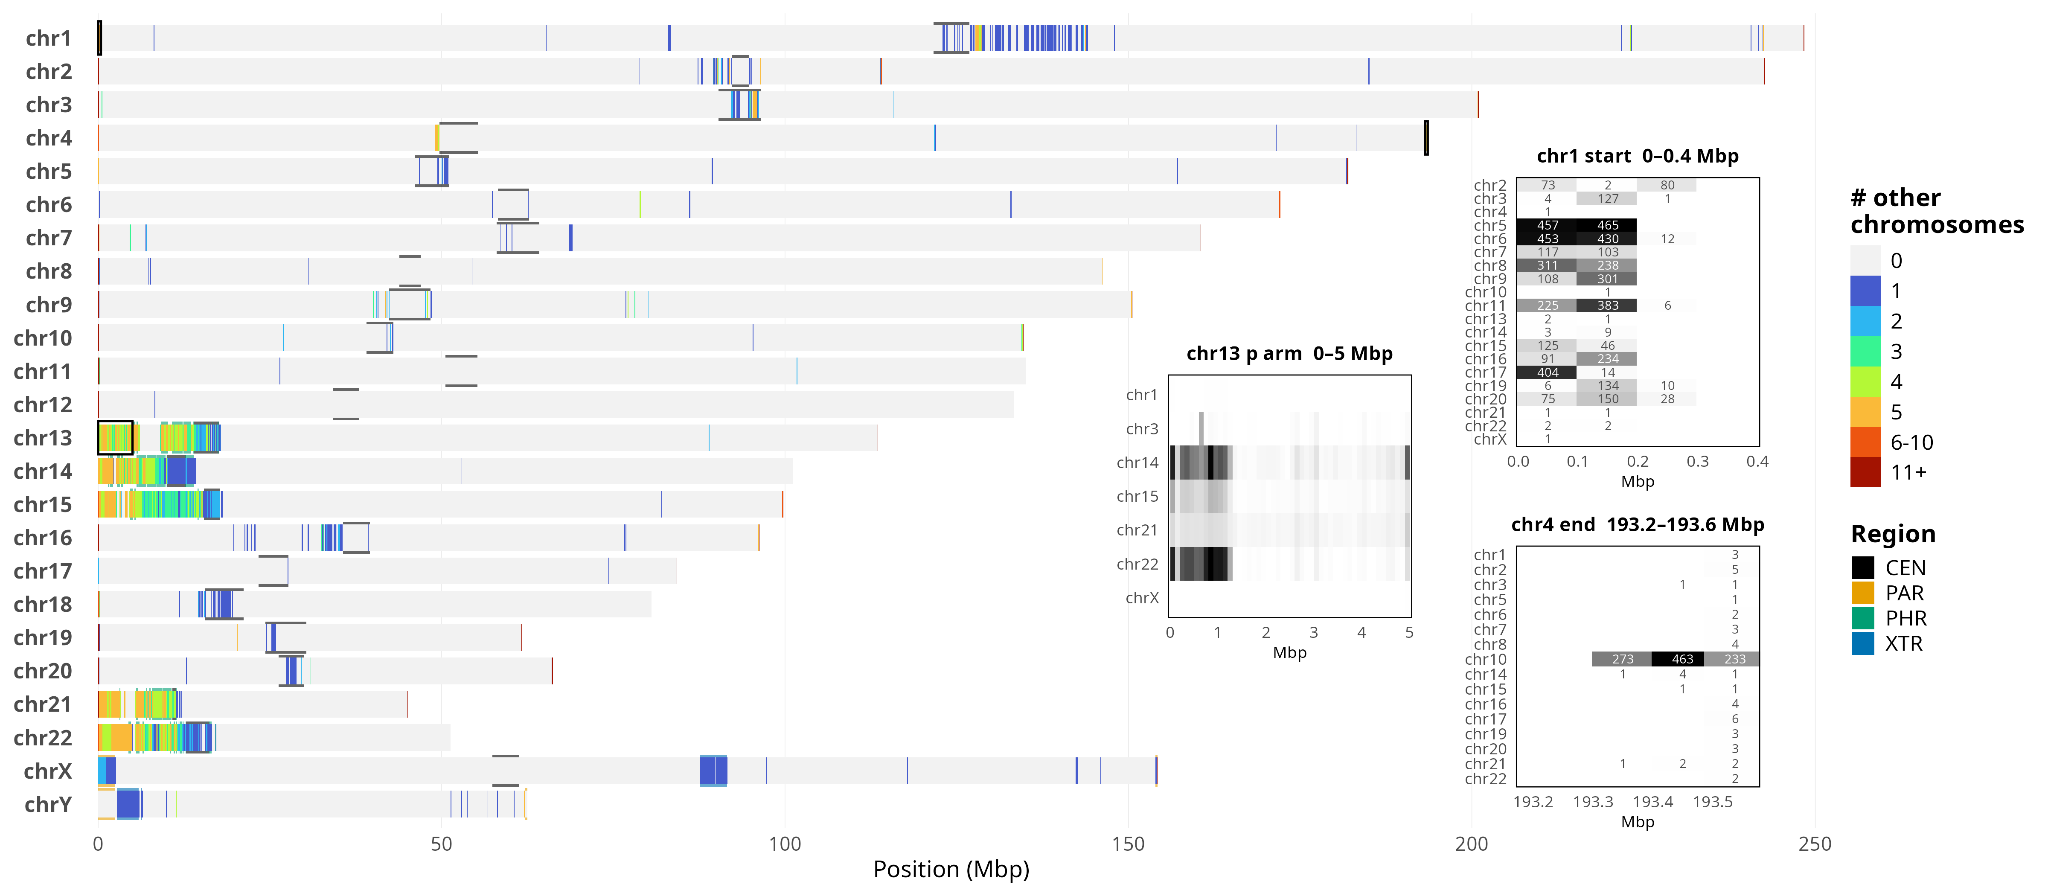
\includegraphics[width=\linewidth]{fig/MainFigures/Fig1a_genomewide.png}\\[4pt]
  
\includegraphics[width=\linewidth]{fig/MainFigures/Fig1b_lengths.png}
  \caption{\textbf{Genome-wide subtelomeric homology and PHR extent.}
    \textbf{(a)} Interchromosomal homology across 465 HPRC v2 haplotypes plus
    CHM13. Each chromosome is shown in 100 kb windows coloured by the number of
    distinct partner chromosomes a window aligns to elsewhere in the pangenome
    (0 to 11+), with a region track (centromere, PAR, PHR, terminal repeat);
    insets give per-partner counts at representative loci. Telomere-anchored
    high-identity blocks mark the inter-chromosomal exchange landscape, and the
    acrocentrics and PARs appear as positive controls.
    \textbf{(b)} PHR length distribution by chromosome end, p-arms and q-arms
    separately, as within-end share per 10 kb bin across the terminal 500 kb
    (q-arms flipped to read telomere$\to$centromere). Non-acrocentric, non-PAR
    PHRs total 3.510 Mb (median 105 kb, mean 144 kb; saturation at 500 kb
    reflects the input flank size, not biology).}
  \label{fig:fig1}
\end{figure}

\begin{figure}[h!]
  \centering
  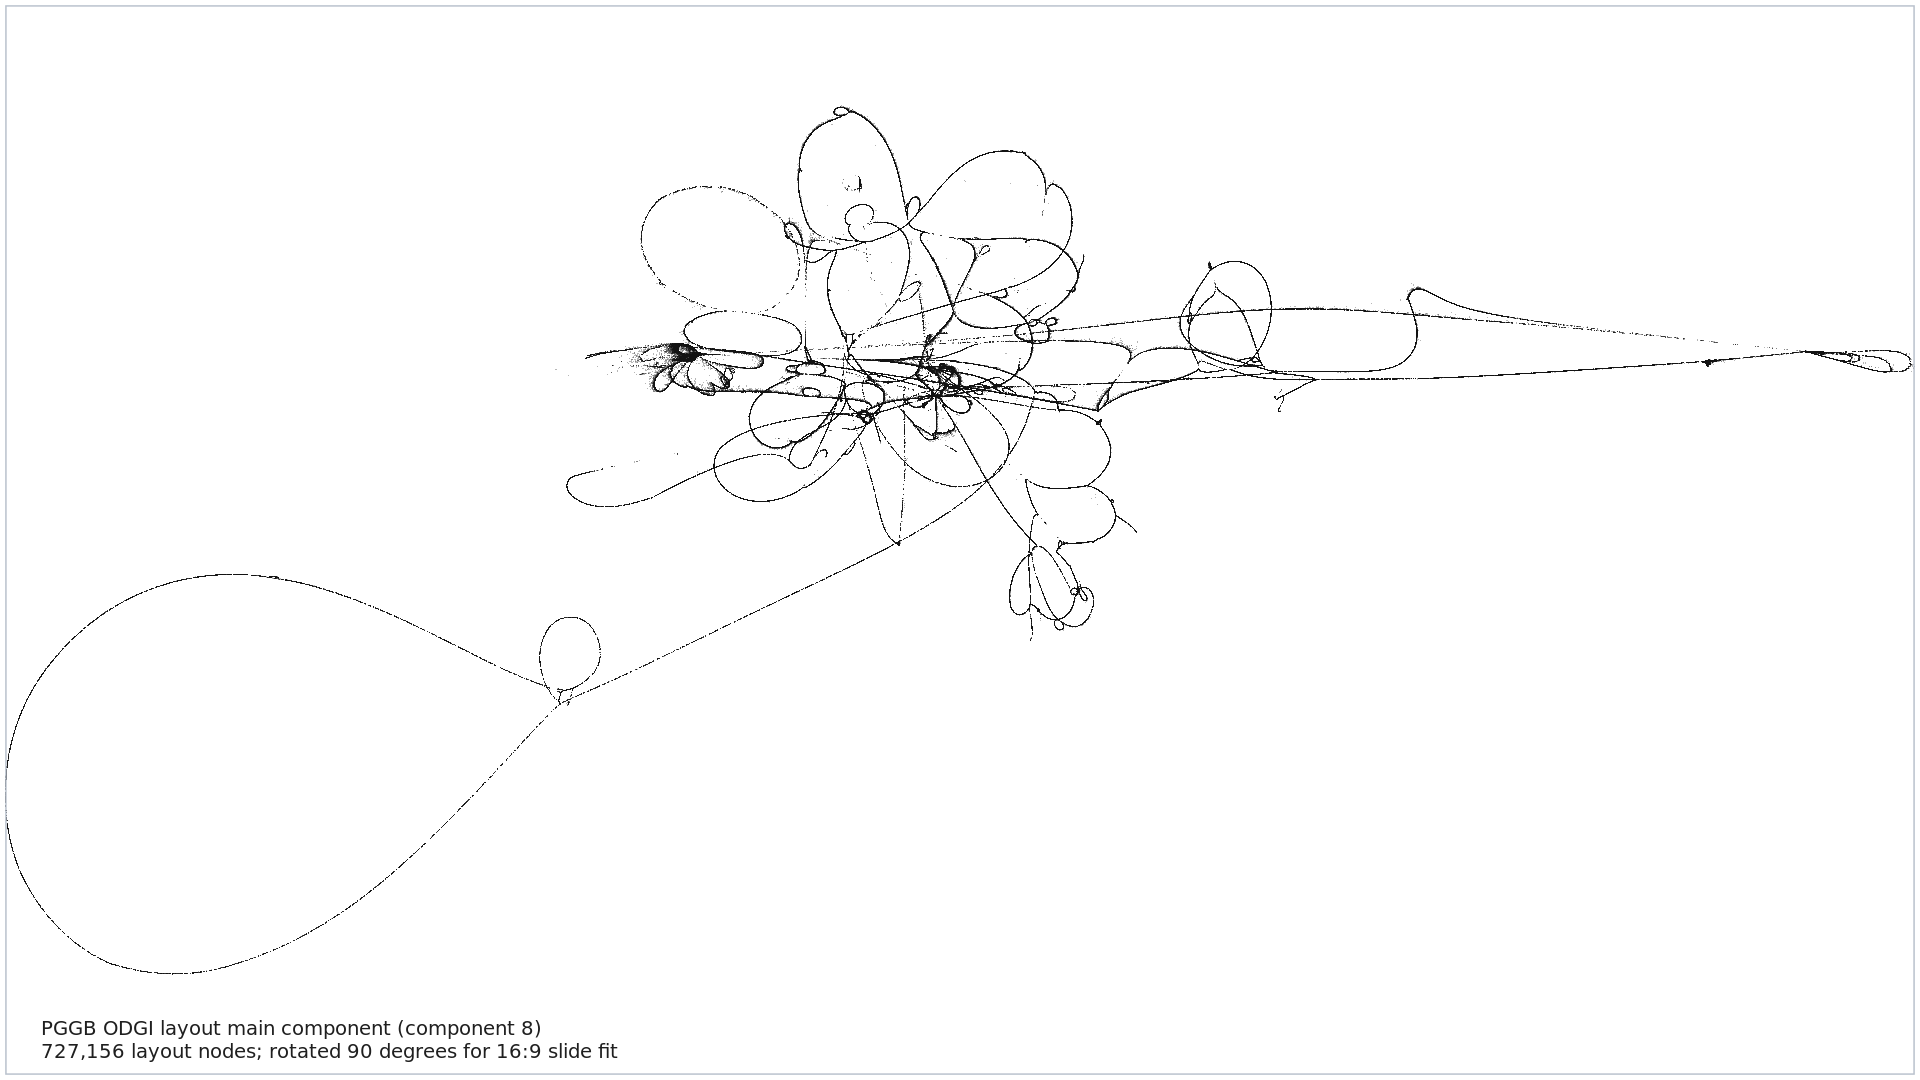
\includegraphics[width=\linewidth]{fig/MainFigures/Fig2a_pggb_layout.png}\\[4pt]
  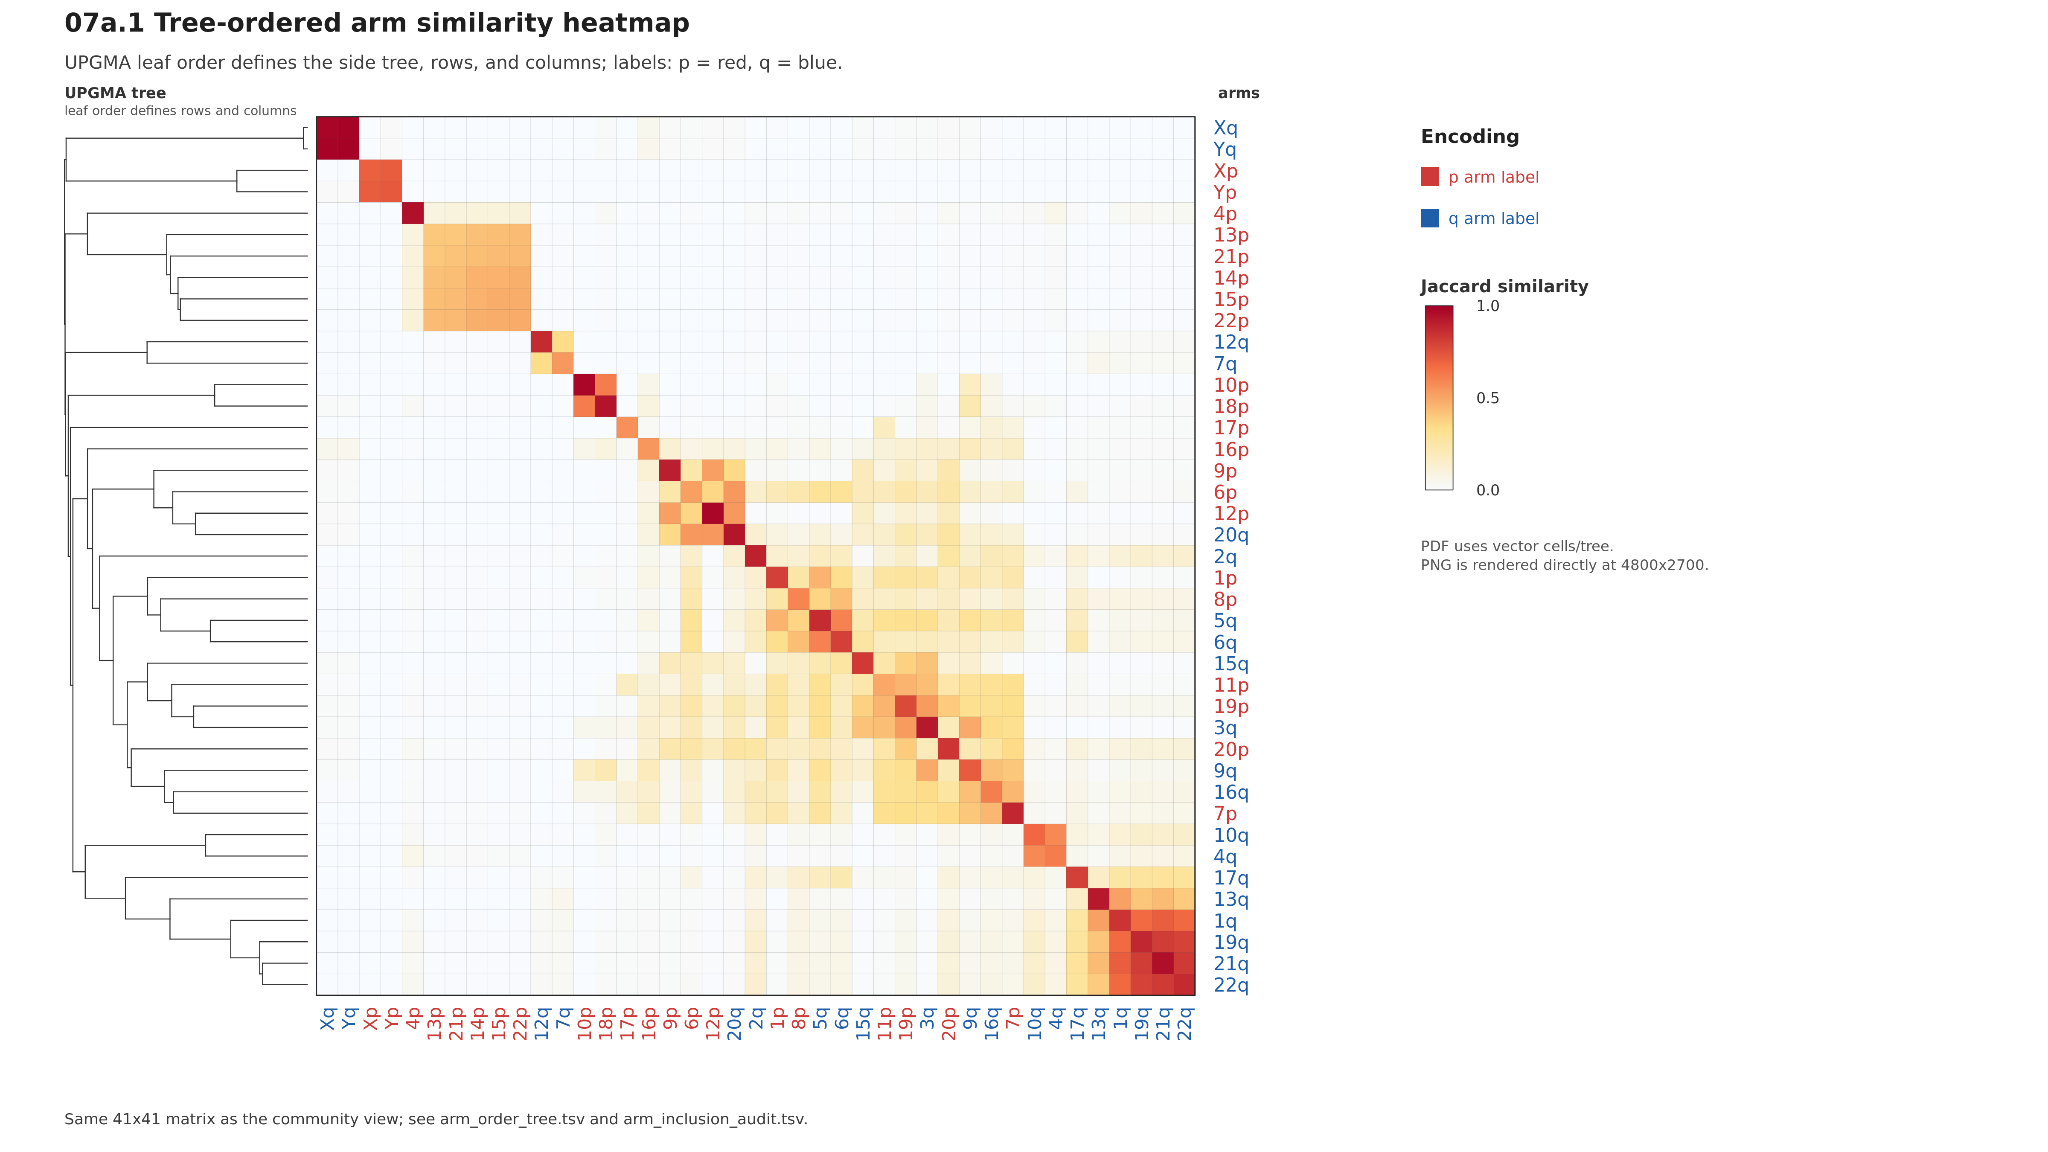
\includegraphics[width=0.49\linewidth]{fig/MainFigures/Fig2b_tree_jaccard.png}\hfill
  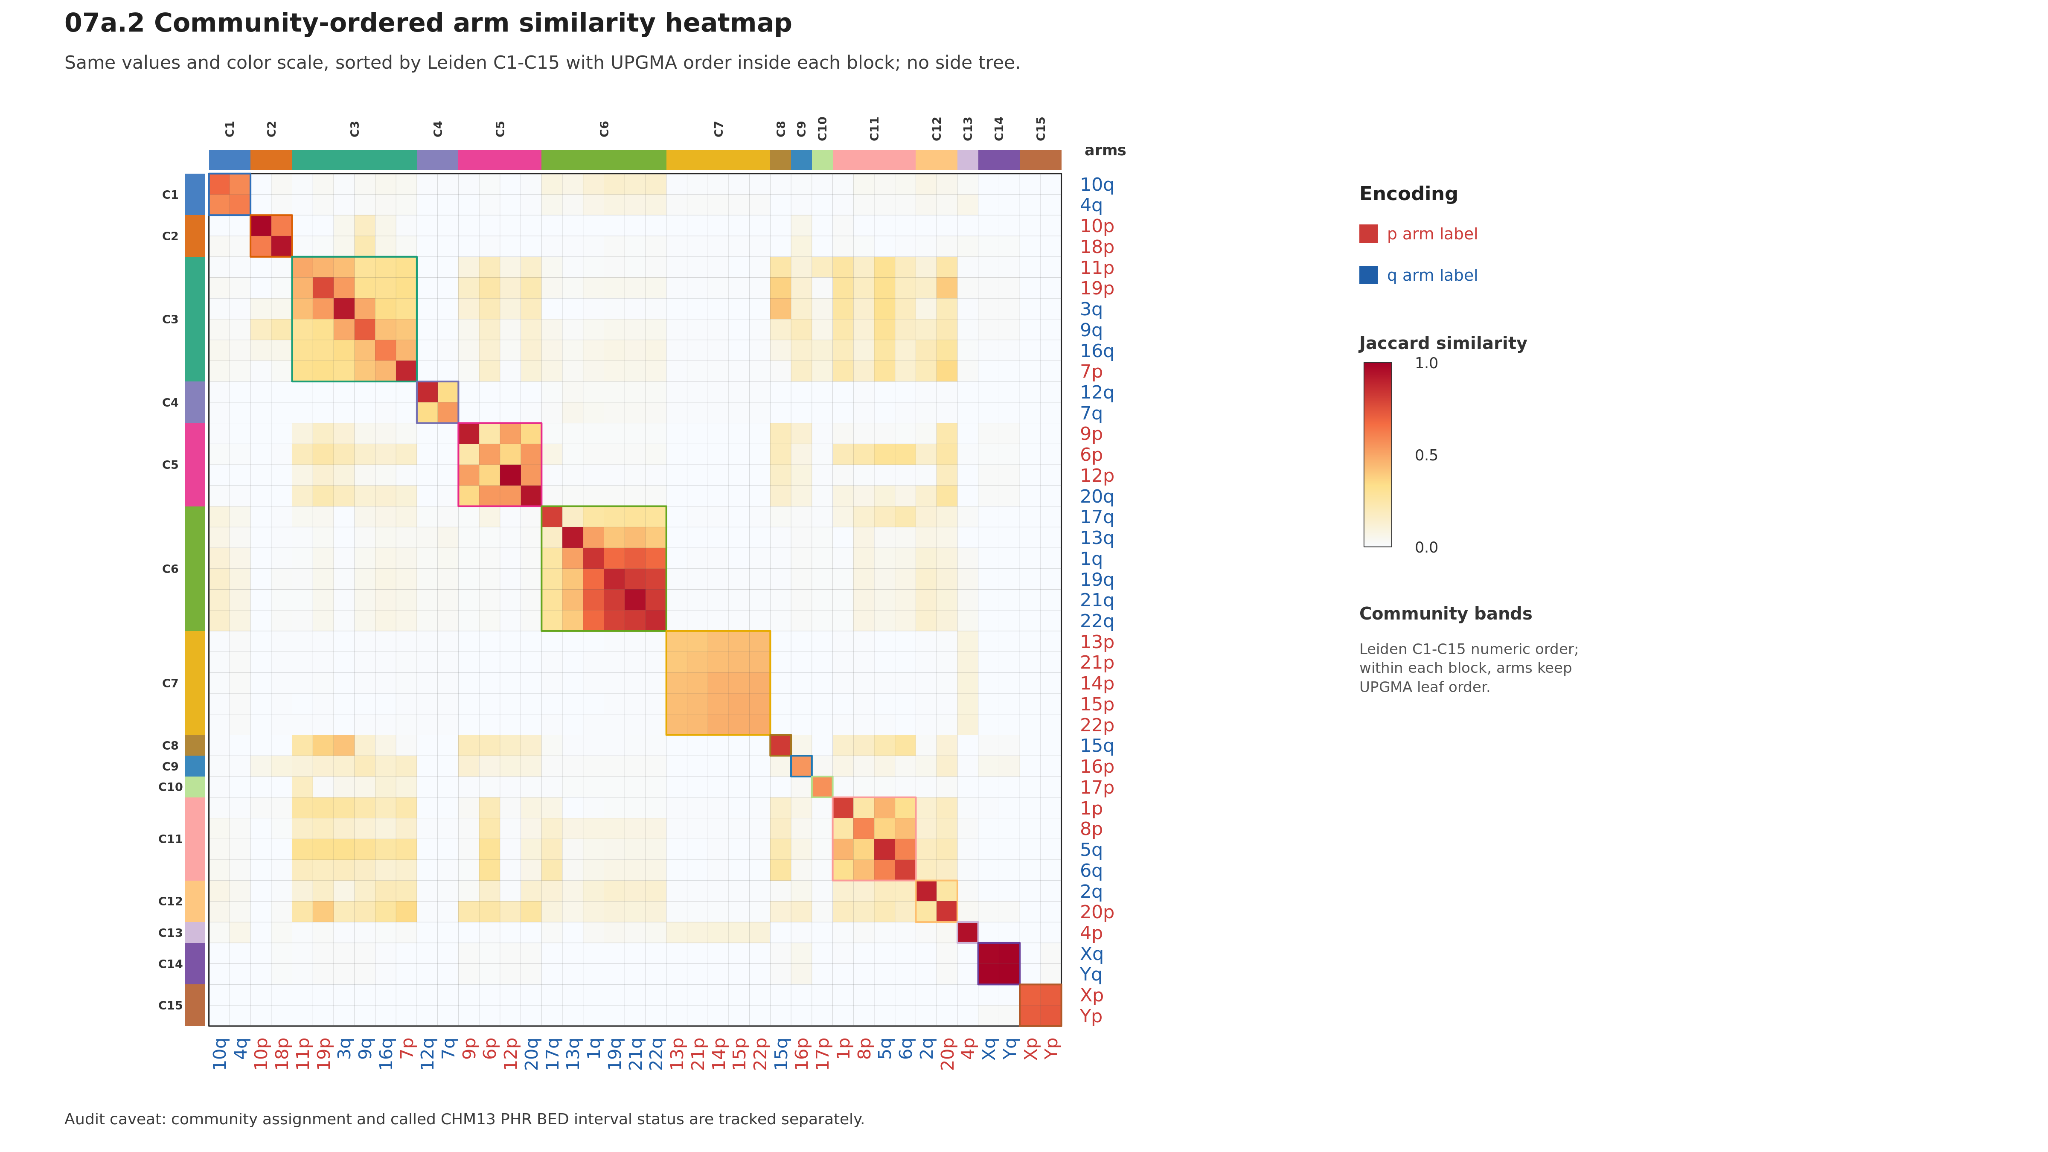
\includegraphics[width=0.49\linewidth]{fig/MainFigures/Fig2c_community_jaccard.png}
  \caption{\textbf{Pangenome similarity structure and communities.}
    \textbf{(a)} PGGB/odgi 2D layout of the all-subtelomere PHR graph (727,156
    layout nodes; main connected component). All 15,668 PHR flanks fall into a
    single component, so subtelomeres are linked across non-homologous
    chromosomes rather than partitioned by chromosome.
    \textbf{(b)} Tree-ordered arm-level Jaccard similarity heatmap
    ($41 \times 41$), leaf order from the UPGMA tree (the ``phylogeny'' of
    subtelomeric PHRs; p-arms red, q-arms blue). The matrix is not a uniform
    gradient but resolves into discrete blocks of co-similar arms.
    \textbf{(c)} The same $41 \times 41$ matrix ordered by Leiden $k = 15$
    community, with community colour bands. The blocks recover every known case
    of inter-chromosomal subtelomere homology: PAR1, PAR2, the acrocentric
    p-arms, 10p/18p, the 4q/10q DUX4 pair, and a tight
    \{22q, 21q, 19q, 1q, 13q, 17q\} q-arm grouping.}
  \label{fig:fig2}
\end{figure}

\begin{figure}[h!]
  \centering
  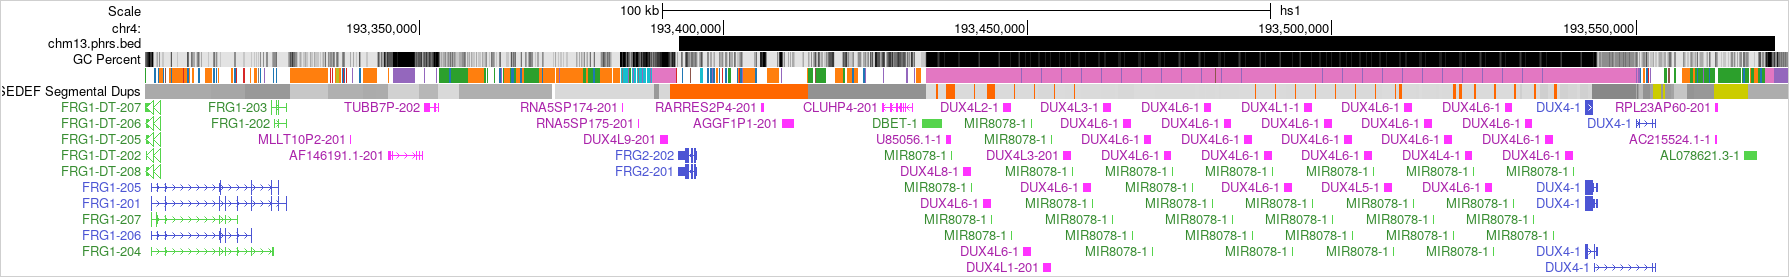
\includegraphics[width=\linewidth]{fig/MainFigures/Fig3a_C1_chr4q.png}\\[1pt]
  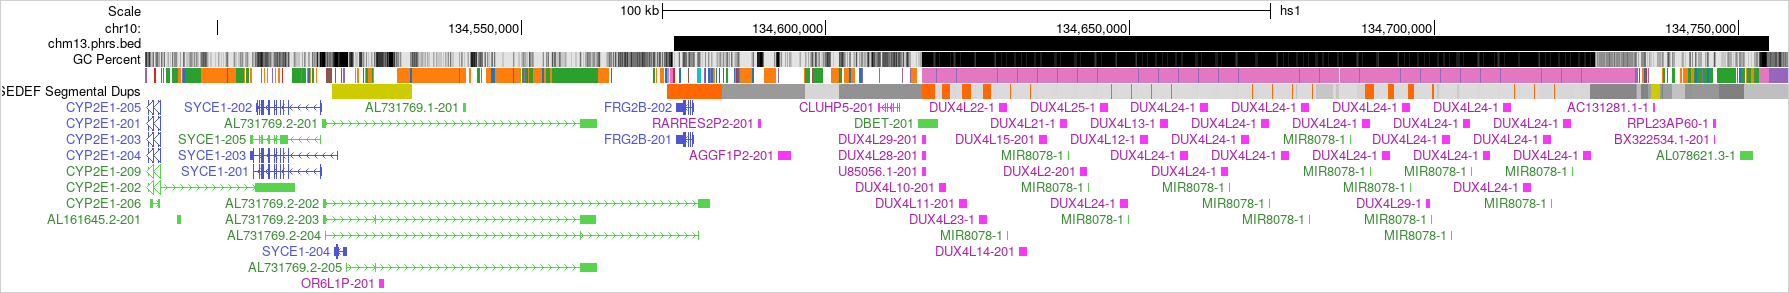
\includegraphics[width=\linewidth]{fig/MainFigures/Fig3a_C1_chr10q.png}\\[5pt]
  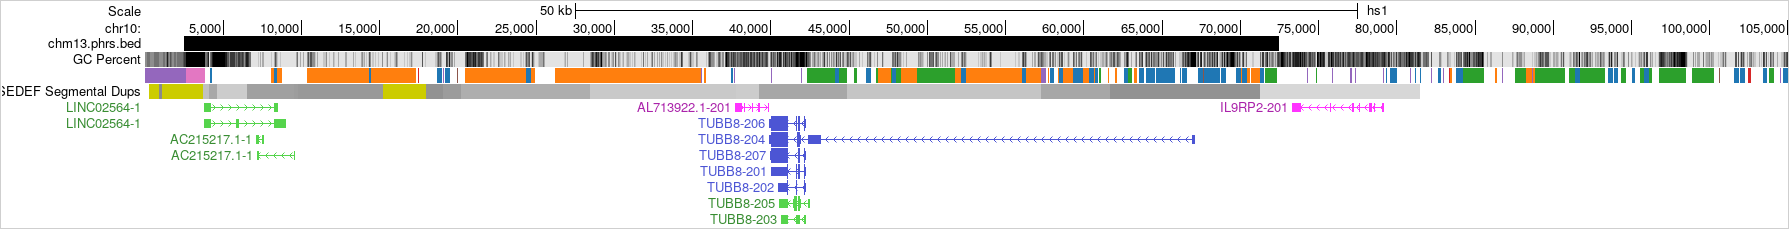
\includegraphics[width=\linewidth]{fig/MainFigures/Fig3b_C2_chr10p.png}\\[1pt]
  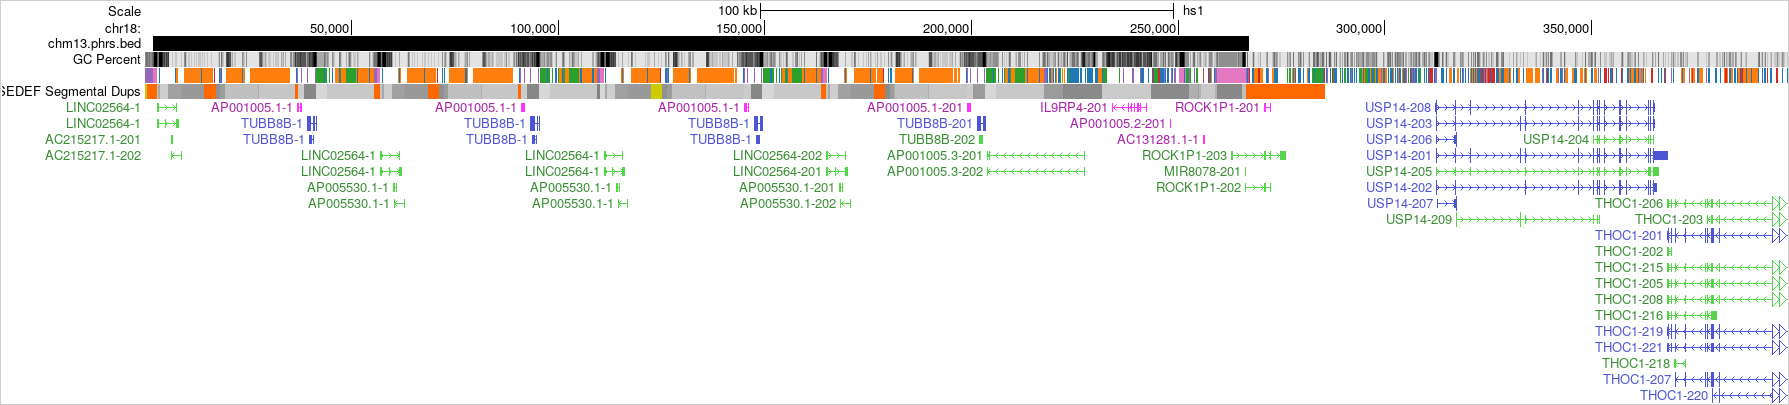
\includegraphics[width=\linewidth]{fig/MainFigures/Fig3b_C2_chr18p.png}\\[5pt]
  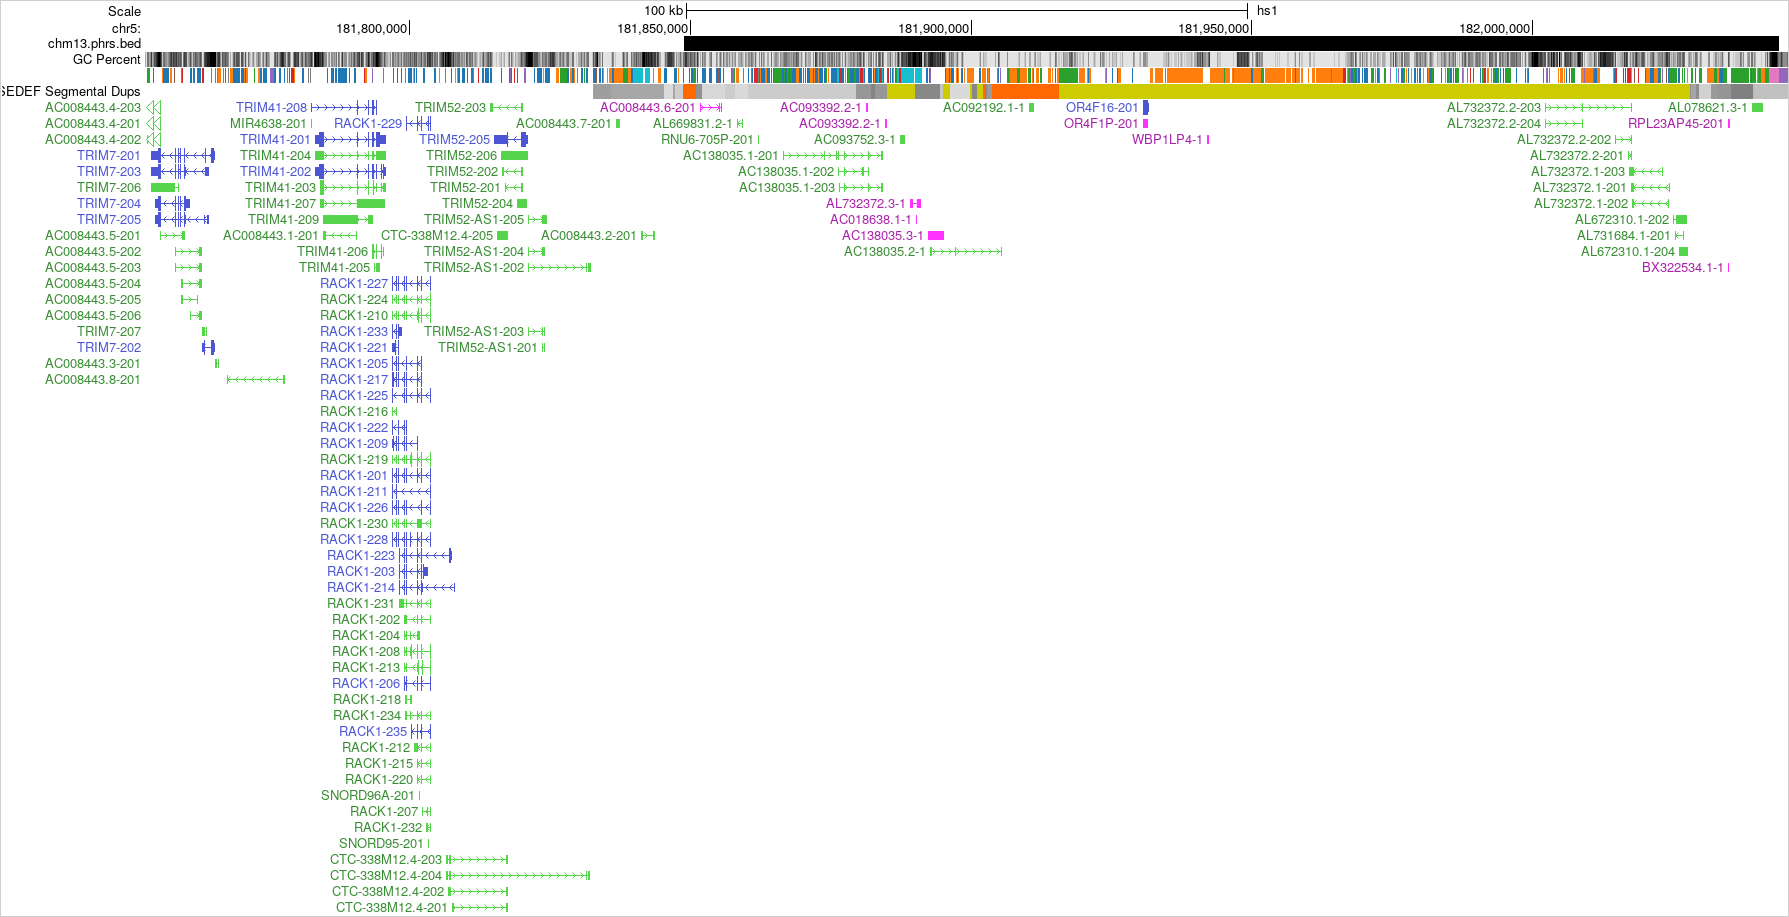
\includegraphics[width=\linewidth]{fig/MainFigures/Fig3c_C11_chr5q.png}\\[1pt]
  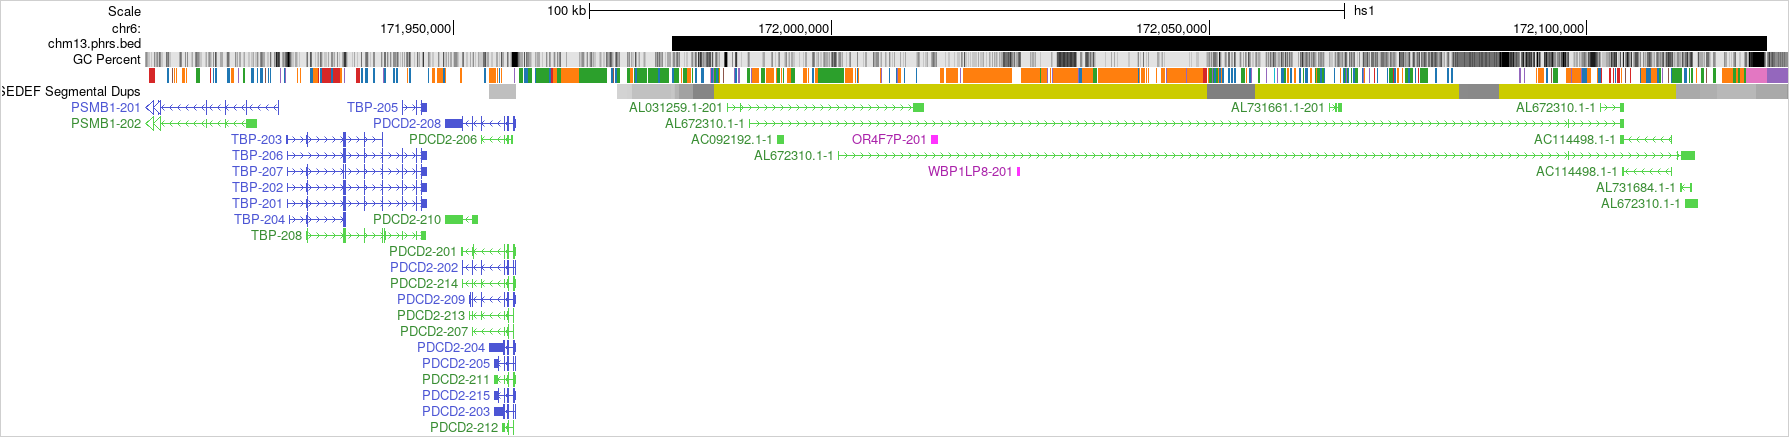
\includegraphics[width=\linewidth]{fig/MainFigures/Fig3c_C11_chr6q.png}
  \caption{\textbf{Architecture of representative communities.}
    Sequence-level views (CHM13 coordinates, with PHR-BED, GC\%, segmental
    duplications and gene models) of three communities, so the duplicon content
    is legible without a genome browser.
    \textbf{(a)} Community C1 (4q/10q), the D4Z4/DUX4 system: homologous DUX4L
    macrosatellite arrays and FRG1/FRG2 paralog families on the 4q35 (top) and
    10q26 (bottom) ends, copy number 0--22 across haplotypes.
    \textbf{(b)} Community C2 (10p/18p), anchored by the TUBB8B tubulin gene
    array (tandem on 10p, top; single-copy on 18p, bottom).
    \textbf{(c)} Community C11 (5q/6q; 5q top, 6q bottom), built on the OR4F
    olfactory-receptor family and its pseudogenes.}
  \label{fig:fig3}
\end{figure}

\begin{figure}[h!]
  \centering
  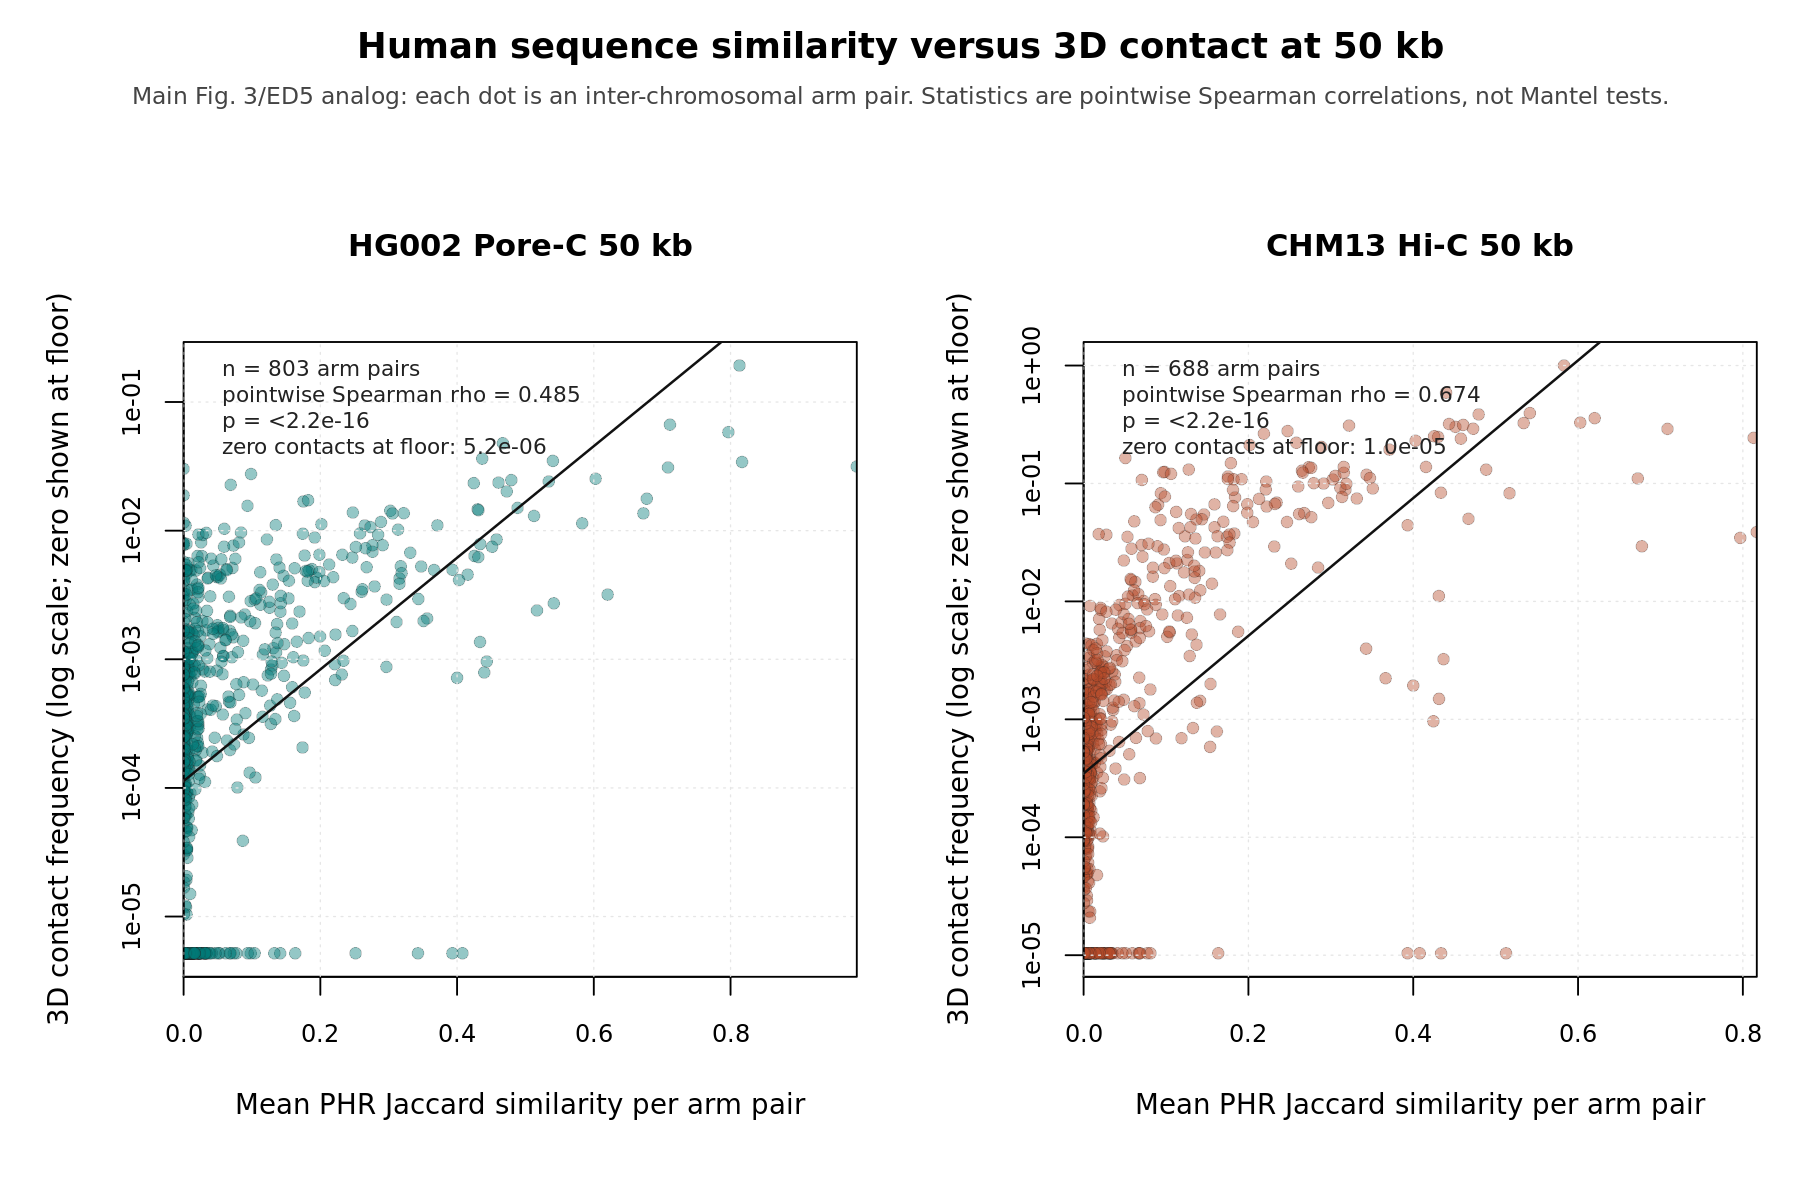
\includegraphics[width=\linewidth]{fig/MainFigures/Fig4a_human_scatter.png}\\[4pt]
  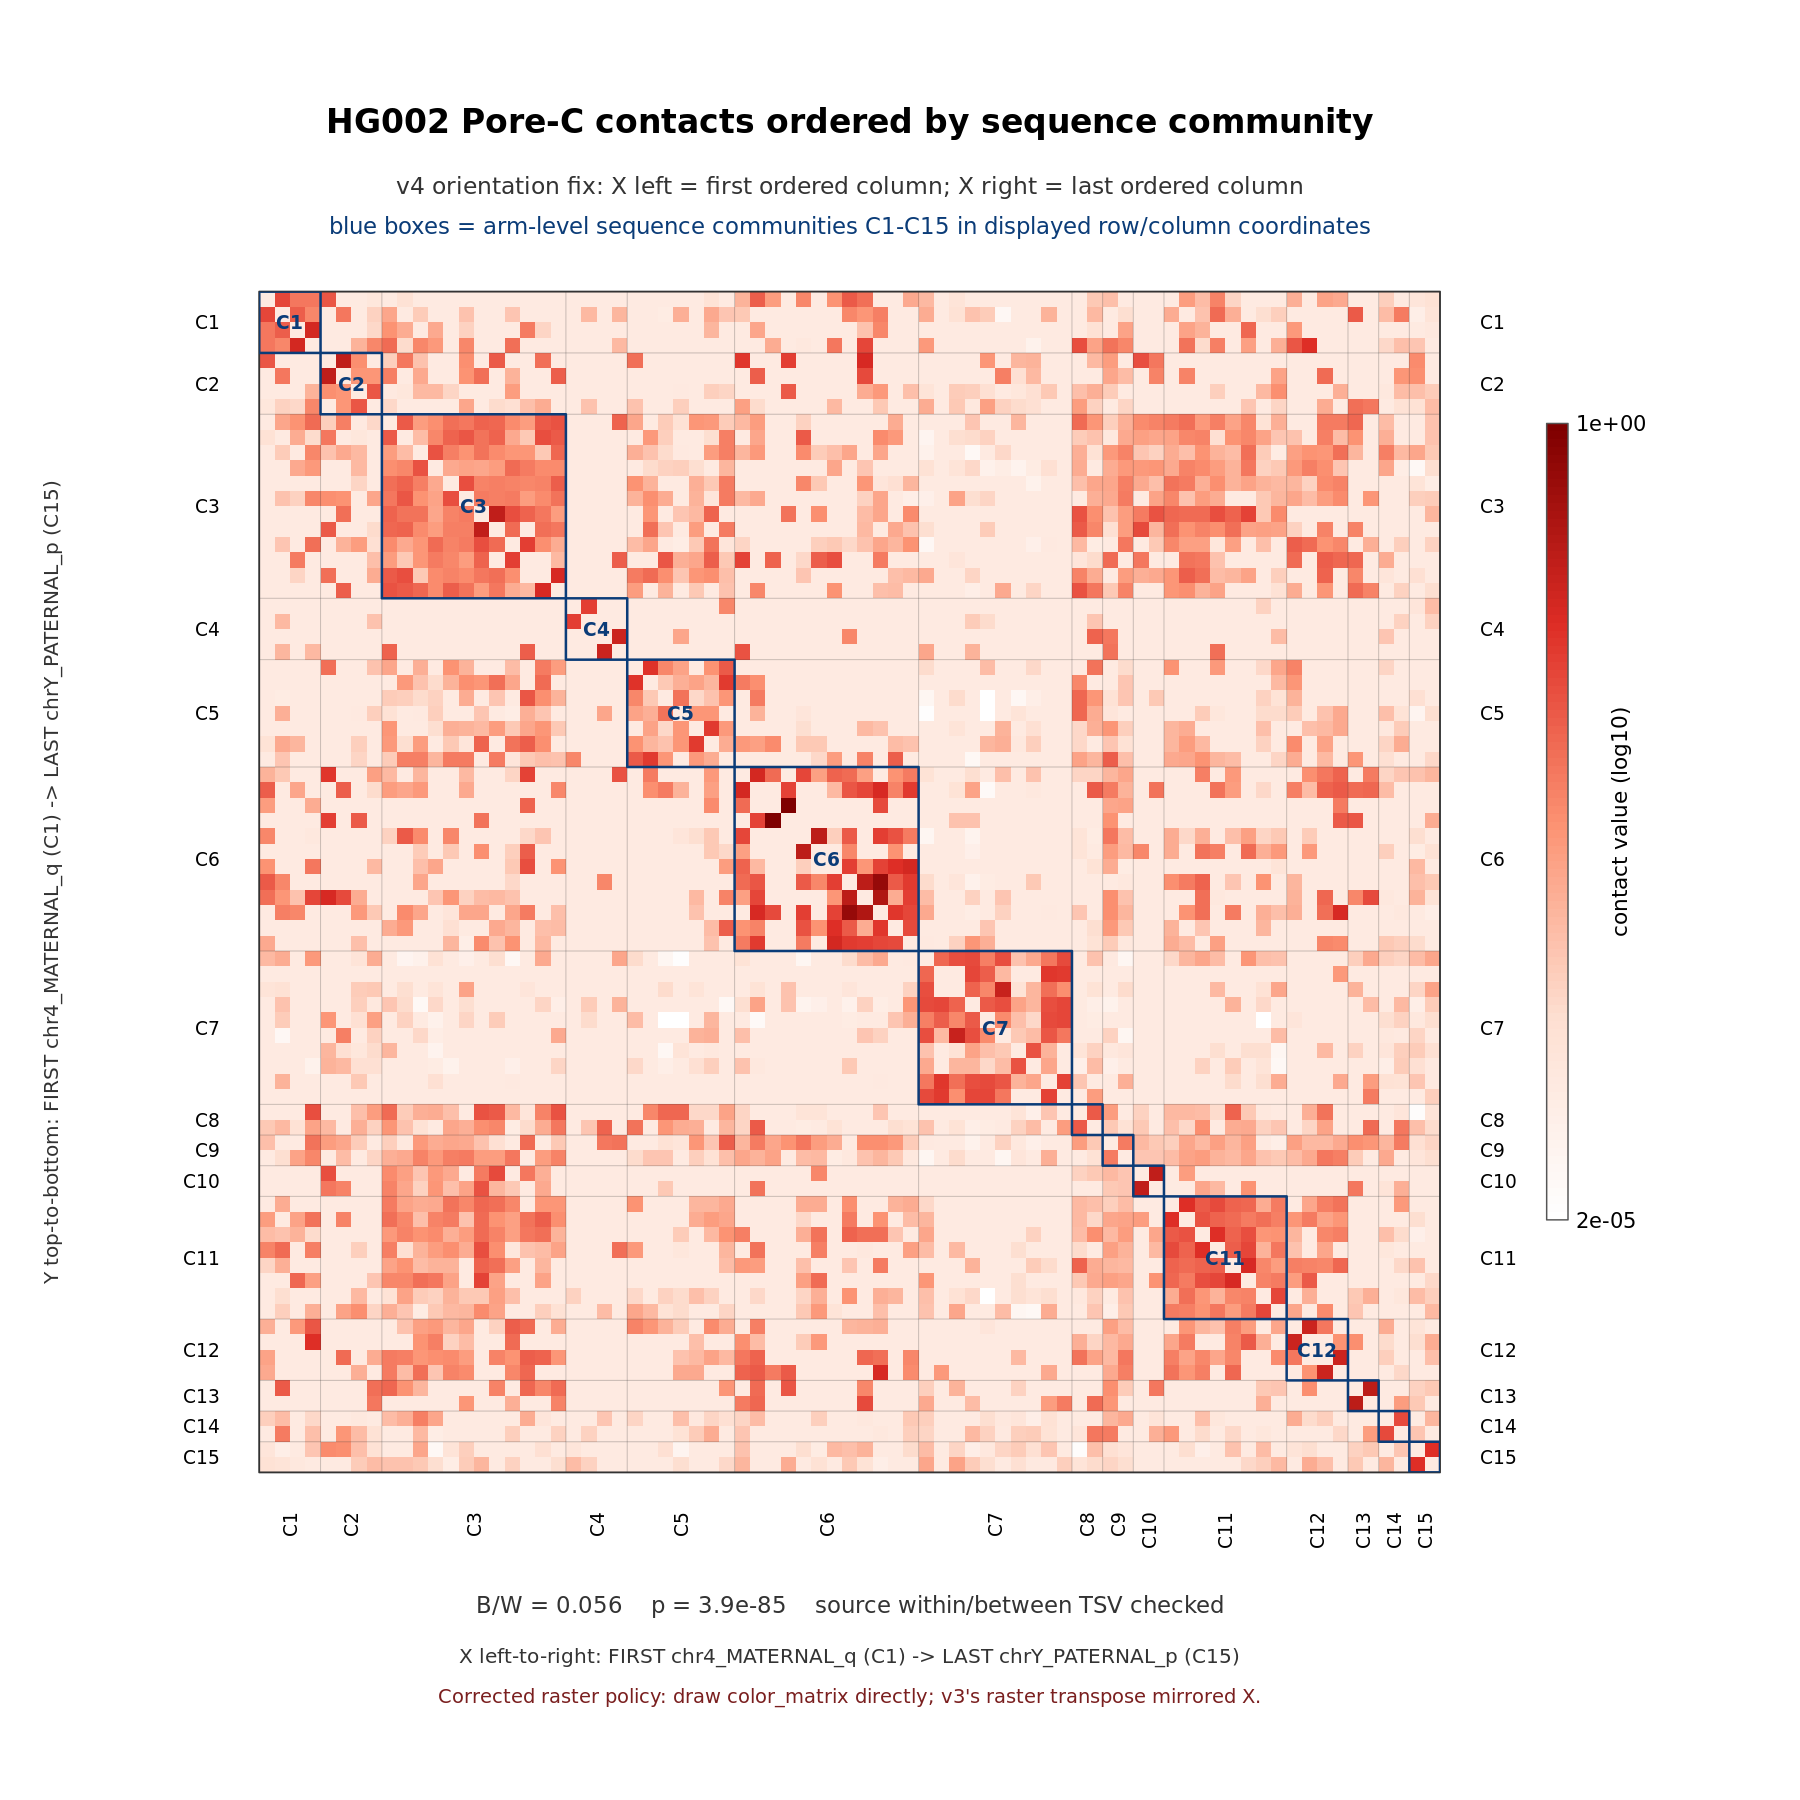
\includegraphics[width=0.6\linewidth]{fig/MainFigures/Fig4b_porec_community.png}
  \caption{\textbf{Sequence similarity predicts three-dimensional proximity.}
    \textbf{(a)} Per arm-pair, three-dimensional contact frequency (log scale)
    vs mean PHR Jaccard similarity at 50 kb, for HG002 Pore-C (pointwise
    Spearman $\rho = 0.485$, $p = 2.2 \times 10^{-26}$, $n = 803$) and CHM13
    Hi-C ($\rho = 0.474$, $p = 2.2 \times 10^{-26}$, $n = 688$).
    \textbf{(b)} HG002 Pore-C contact matrix ordered by sequence community
    (C1--C15): within-community blocks dominate, $B/W = 0.056$,
    $p = 3.9 \times 10^{-85}$.
    The mouse meiotic-stage analogue (zygotene bouquet), which lacks a human
    germline-stage equivalent and validates the Hi-C pipeline, is shown in
    Extended Data Fig.~\ref{fig:ed1}.}
  \label{fig:fig4}
\end{figure}

\begin{figure}[h!]
  \centering
  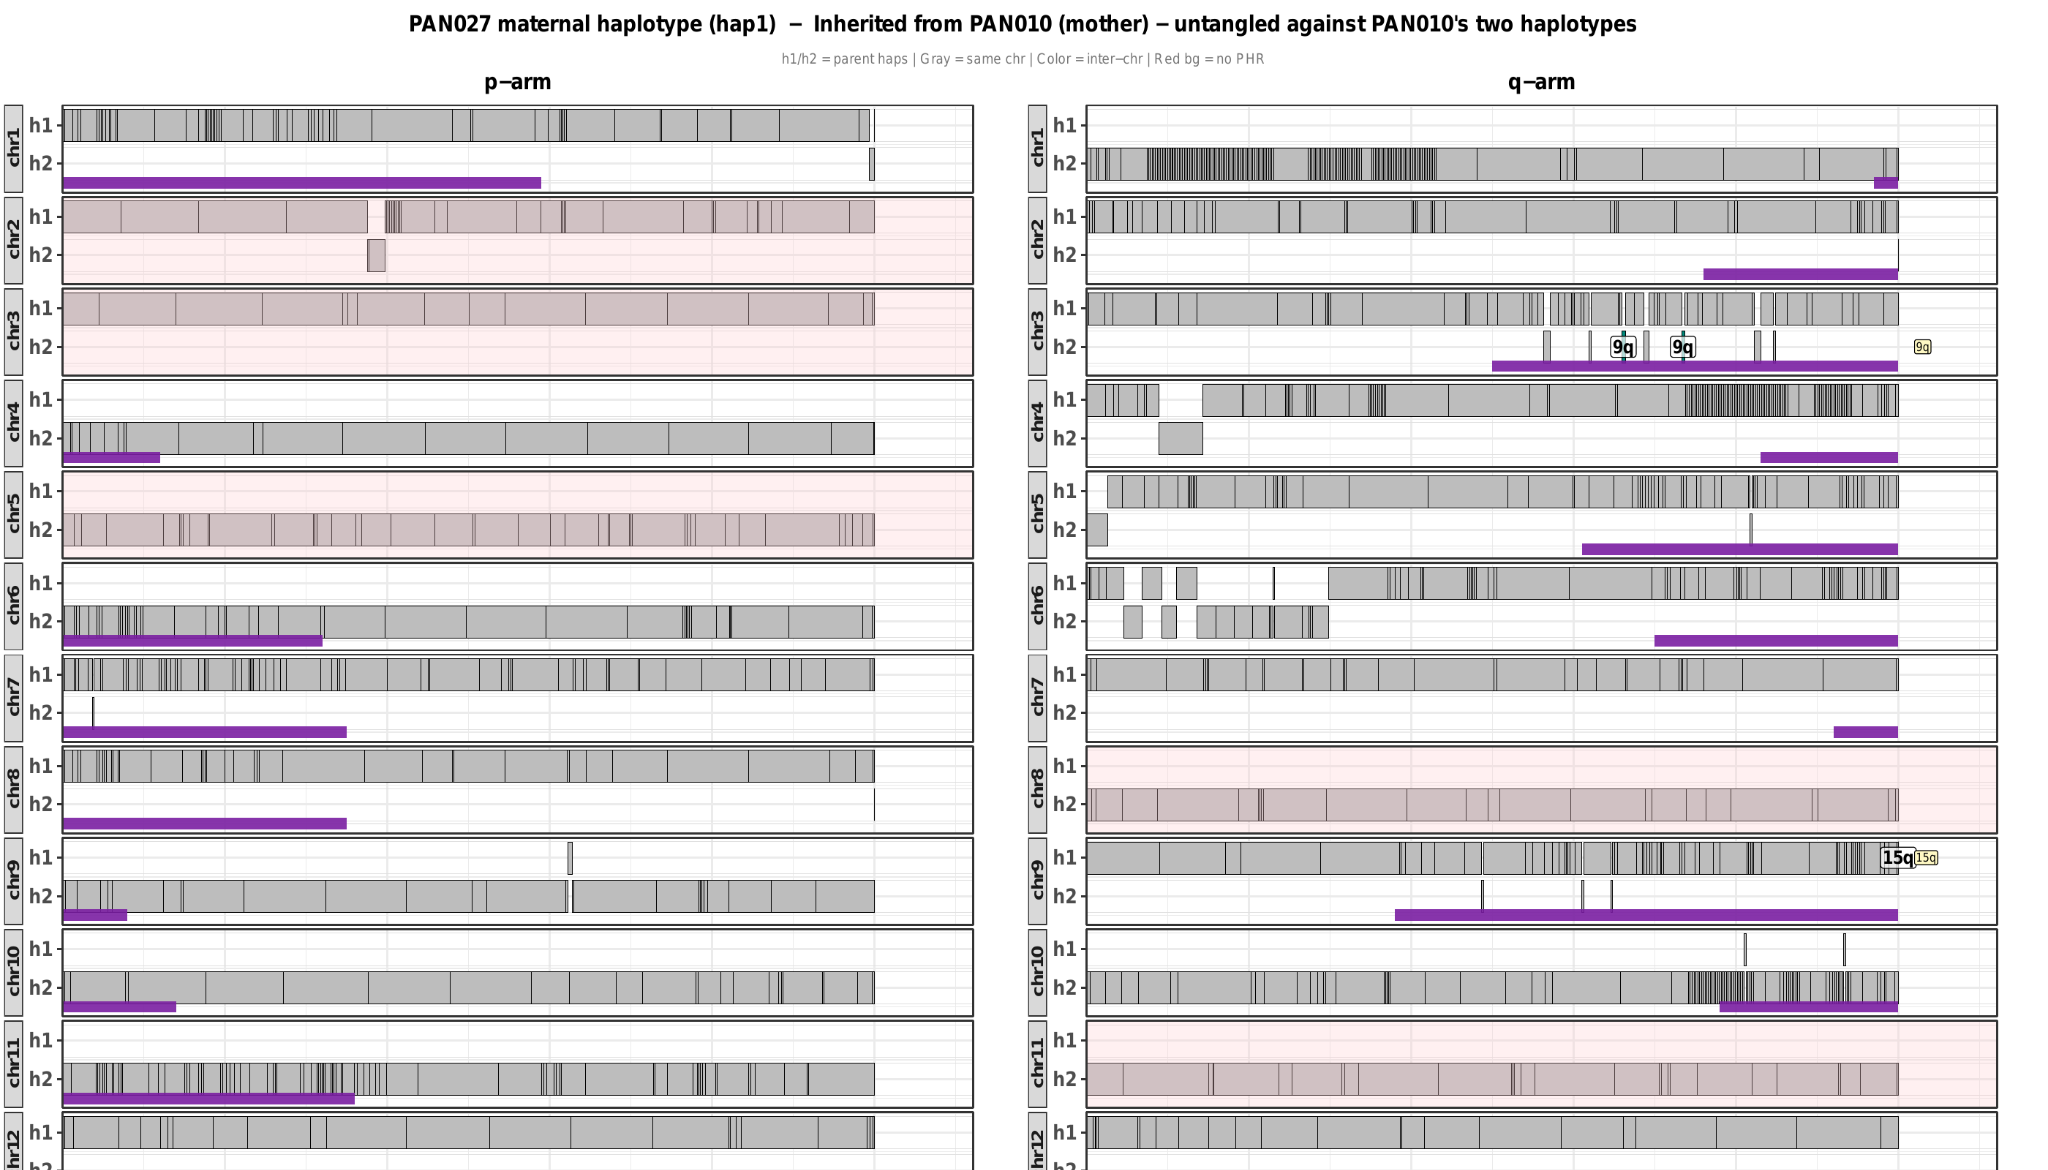
\includegraphics[width=\linewidth]{fig/MainFigures/Fig5_pedigree_untangle.png}
  \caption{\textbf{Pedigree-resolved subtelomeric exchange.}
    Inter-chromosomal recombination caught in the act in the WashU
    three-generation T2T pedigree. The PAN027 maternal haplotype (hap1,
    inherited from the mother PAN010) is untangled against PAN010's two
    haplotypes with \texttt{odgi untangle}, per chromosome arm (p-arms left,
    q-arms right; purple bars mark inter-chromosomal patches). Of 538
    high-quality patches, 494 (92\%; Wilson 95\% CI 89.2--93.9\%) fall within a
    sequence-similarity (Leiden) community, above a marginal-aware Monte Carlo
    null (mean 77.0\%, 95\% CI 75.4--78.8\%; $p < 10^{-4}$), including
    crossover-like reciprocal exchanges and perfect-identity gene-conversion
    tracts. Cross-assembler validation (CEPH1463) and the RPE-1 t(X;10)
    positive control are described in the main text.}
  \label{fig:fig5}
\end{figure}

\section*{Methods}
\label{secMethods}

\setcounter{figure}{0}

\subsection*{Sample selection and reference frame}

233 HPRC v2 v1.1 individuals contributed haplotype-resolved assemblies, and
CHM13v2.0 was added as the closed-reference anchor.
The arm-flank census uses 465 haplotypes (233 samples $\times$ 2, minus 1
because CHM13 contributes a single haploid sequence).
Superpopulation breakdown: AFR 67, EAS 52, AMR 44, SAS 37, EUR 33
\citeMeth{hprc_hprcv2_2025,Nurk2022,logsdon2025hgsvc}.

\subsection*{Sample exclusions}

Two exclusions are applied.
(i) GRCh38 contigs and CHM13\#0\#chrY (masked PAR1) are excluded from flank
extraction because they carry no telomeres compatible with the 500 kb anchored
extraction (\texttt{01\_pipeline.md} \S Flank extraction).
(ii) The chr18\_q flank from NA18982\#1 (JBKABS010000018.1, 84.4 Mb) is
excluded as a scaffolding chimera that fuses chr18 with 966 kb of chrX PAR1
across an NNN gap; confirmed by both wfmash and minimap2 v2.30 at MAPQ 60 and
by Flagger NNN/Hap labels (\texttt{01\_pipeline.md} \S Chimeric contig
exclusion).
No additional haplotype-level exclusions are applied.

\subsection*{Telomere-anchored 500 kb flank extraction}

For each haplotype assembly we extracted the terminal 500 kb of every contig
classified as p- or q-arm telomere-bearing (contig length $\geq 1$ Mb),
producing 18,827 flanks across 48 arms.
pq-classification at \texttt{pq-classification/contig\_classifications.tsv}.

\subsection*{wfmash all-vs-all alignment}

\texttt{wfmash v0.23.0-41-gb5f0ff1c -p 95 -t 48 --quiet}; each flank serves
as target in turn \citeMeth{Guarracino2023}.
In a panmictic population most pairwise alignments are redundant; transitive
closure of the sampled fraction recovers effectively the same sequence graph as
exhaustive all-vs-all alignment.

\subsection*{Implicit pangenome graph and IMPG transitive closure}

The all-vs-all PAF set is the implicit pangenome graph; IMPG \texttt{query -x}
computes reachability
\citeMeth{pangenome_graphs_impg_GuarracinoHeumos2022,pangenome_graphs_impg_Hickey2024}.
Realised sampling rate 11.6\% (12\% rounded) sits $230\times$ above the
Erd\H{o}s and R\'{e}nyi connectivity threshold
$p^{*} = \log(n)/n = 5.2 \times 10^{-4}$ for $n = 18827$, justifying the
absence of chromosomal partitioning.

\subsection*{PHR detection}

IMPG sliding-window scan: identity $\geq 95\%$, $\geq 5$ alignments per
chromosome on $\geq 2$ different chromosomes, total aligned length per window
$\geq 3$ kb.
Output: 15,668 PHRs (83.2\% of flanks), 41 of 48 arms \citeMeth{Garrison2018}.

\subsection*{Pangenome graph and Jaccard similarity}

\texttt{pggb -p 95 -D /scratch}; \texttt{odgi similarity --all -P} over the
15,668 sequences yields the $15668 \times 15668$ Jaccard matrix
\citeMeth{Garrison2024pggb,andreace2023pangenome,heumos2024nfcore}.
The single connected component is rendered with \texttt{odgi layout} +
\texttt{odgi draw} (Fig.~\ref{fig:fig2}a).

\subsection*{Arm-level distance matrix}

Mean pairwise sequence-level Jaccard distance within each arm pair
(\texttt{hprcv2.1Mb.subtelo.arm\_dist\_matrix.tsv}).

\subsection*{Community detection (Leiden)}

Arm-level: edge weight $w_{ij} = \exp(-d_{ij} / \text{median}(d))$; resolution
scanned 0.1--3.0 at 0.01 step; selected resolution 1.16 (mean silhouette
0.347, $k = 15$).
Sequence-level: k-NN graph with $k \in \{10, 25, 50, 75, 100, 125\}$ and
resolution 0.1--3.0; selected $k = 75$, resolution 0.8 (modularity 0.97, mean
silhouette 0.602, $k = 50$).

\subsection*{UPGMA dendrogram}

\texttt{hclust(..., method = "average")}; $k = 14$ (mean silhouette 0.342);
agreement with Leiden 12 of 15.

\subsection*{Neighbour-joining tree and character-level bootstrap}

\texttt{ape::nj()} on the $41 \times 41$ arm-level Jaccard distance matrix;
rooted at the MRCA of the acrocentric grouping.
Support from a 1,000-replicate character-level bootstrap
(\texttt{scripts/cladistics/char\_bootstrap\_d\_m9.R}): each replicate
resamples PHR flanks with replacement, rebuilds the arm-level distance from
cached per-PHR cross-chromosome involvement (no PGGB re-run; $\approx 108$ s
single-core), and recomputes NJ + UPGMA.
Per-grouping support: PAR1/PAR2/10p18p 100\%, 4q/10q DUX4 99.4\% NJ,
acrocentric p-arms 52\% NJ / 87\% UPGMA; the 6-arm tight q-arm grouping is
0.1\% because the per-PHR involvement column is chromosome-granular (conflating
the q-grouping with chr2\_q and chr10\_q); resolving it at the character level
requires the per-arm-pair PGGB closure and is deferred.
NJ used as an ordering device, not a phylogenetic claim.

\subsection*{Heterogeneity tests}

Wilcoxon paired test (allele vs paralog); per-arm Spearman correlation between
chromosome contributors and distance from telomere; piecewise regression with
changepoint detection; $2 \times 5$ Fisher exact test for cross-arm vs
self-arm superpopulation composition with BH correction; Hudson pairwise
$F_{\mathrm{ST}}$ \citeMeth{subtel_popgen_hudson1992,subtel_popgen_weir1984}.

\subsection*{$F_{\mathrm{ST}}$ and population structure}

Hudson $F_{\mathrm{ST}}$ values 0.10--0.15 between AFR and each non-AFR
superpopulation ($-0.05$ to 0.01 within non-AFR) sit within the genome-wide
continental range \citeMeth{subtel_popgen_bhatia2013}.
Block-jackknife 95\% CIs leave-one-arm-out over 9 arm/community blocks passing
Fisher $p_{\mathrm{adj}} < 0.05$ ($z = 2.306$, d.f.\ = 8): AFR-AMR 0.108
[0.026, 0.191], AFR-EAS 0.155 [0.076, 0.234], AFR-EUR 0.128 [$-0.020$,
0.275], AFR-SAS 0.112 [$-0.001$, 0.224].
Compared against matched 1000G/HGDP continental Hudson $F_{\mathrm{ST}}$
\citeMeth{subtel_popgen_bhatia2013}, all four AFR-vs-non-AFR baselines lie
inside the subtelomeric CI; non-AFR pairs equivalent or depressed; none
elevated.
Analysis: \texttt{scripts/popgen/matched\_fst\_d\_m6.py};
\texttt{scripts/ci/bootstrap\_ci\_d\_m12.\{py,R\}}.

\subsection*{Hi-C, Pore-C and CiFi pipeline}

mcool inputs at 5, 10, 20, 50 and 100 kb; per-haplotype mode preserves
maternal and paternal contigs as separate arms.
MAPQ filters disabled to retain multi-mappers, with one random alignment per
read.
This random-placement approach is an acknowledged limitation rather than a
validated method: the flanking unique-sequence control refutes the multi-mapping artefact in PHR-internal regions
but does not bound a possible bias from uniform MAPQ0 distribution across
paralogous arms within the same community.
Lower-bound estimates of within-community contact are therefore the 9-fold-stronger
flanking values (PHR $B/W = 0.027$ vs flanking $B/W = 0.0031$ in HG002), and
PHR-window B/W ratios should be read as the inflated upper bound on the
artefact-controlled signal rather than the true 3D-contact estimate.
The flanking unique-sequence control operationalises the MAPQ-strict comparison:
across 7 of 7 Hi-C and Pore-C datasets, flanking B/W is 1.25--13.5$\times$
stronger than PHR B/W, falsifying multi-mapping-driven inflation.
A strict-MAPQ re-binning from upstream \texttt{.allValidPairs} (both mates
MAPQ $\geq 30$; \texttt{scripts/hic/mapq\_strict\_d\_peerq1.py}) reproduces the
flanking B/W within Poisson noise while PHR-internal contact collapses to a
noise floor; observed-over-expected normalisation handles the rare
inter-chromosomal regime without random-ligation inflation.
W/B ratio computed by bootstrap on 10,000 permutations; Mann-Whitney global
test; Mantel Spearman with 10,000 row+column permutations; observed-over-expected
inter-chromosomal normalisation
\citeMeth{hic3d_dixon2012,hic3d_imakaev2012,Ulahannan2019,hic3d_cifi2025}.
The per arm-pair pointwise Spearman correlations of Fig.~\ref{fig:fig4}a (HG002
Pore-C $\rho = 0.485$, $n = 803$; CHM13 Hi-C $\rho = 0.474$, $n = 688$) and the
community-ordered Pore-C matrix of Fig.~\ref{fig:fig4}b ($B/W = 0.056$) are
computed at 50 kb.

\subsection*{Reproducibility from deposited data}

Standard deposited Hi-C MCool/Juicer files (default MAPQ $\geq 30$) do not
preserve the inter-arm signal because the high-identity PHR sequence is masked
at the deposited mapping stage.
We re-aligned all Hi-C, Pore-C, CiFi and Dip-C data from raw FASTQ against the
corresponding T2T reference (CHM13v2.0 or matched HPRC v2 haplotype) with
multi-mappers retained.
Re-alignment scripts and command lines are at \texttt{scripts/hic-realign/}.
Anyone attempting to reproduce these results from existing deposited processed
files at default parameters will see no signal.

\subsection*{Exclusion controls (multi-resolution Mantel walk)}

Five exclusion sets (no acrocentric p-arms, no sex chromosomes, no acrocentric
p plus sex, no all-acrocentric plus sex, no strongest community) applied at all
five mcool resolutions.
The resulting Mantel $\rho$ trajectory rises with confound removal: HG002
$0.66 \to 0.80$, HG02148 $0.15 \to 0.72$, CHM13 $0.66 \to 0.85$, NA19036
$0.27 \to 0.79$
\citeMeth{hic3d_alavattam2019,hic3d_wolff2018,hic3d_deshpande2022}.

\subsection*{Single-cell 3D}

Dip-C in 16 GM12878 cells \citeMeth{Tan2018} (17 raw cells; cell 12 excluded as
a duplicate of cell 10 by shared SRR7226706 long-insert library) remapped to
T2T-CHM13v2.0; sperm scHi-C in 20 cells
\citeMeth{Xu2025,hic3d_scnanoHiC2023,hic3d_scnanoHiC2_2025,hic3d_kitamura2025}.
PBMC Dip-C negative control: 18 cells with PHR coordinates projected from
CHM13 to hg19 via impg, yielding $W/B = 0.983$, $p = 0.305$
(\texttt{05\_hic\_validation.md} \S PBMC, L455-469).
$S_{\mathrm{all}}$ negative control: pooled 7 zero-signal arms.

\subsection*{Mouse pipeline}

Repetition of the project on a non-human mammal.
B6 and CAST T2T assemblies \citeMeth{Francis2025}; telomere-anchored flanks;
1/2/4 Mb window sweep (30/49 mouse PHRs saturate the 1 Mb window);
2-community arm-level partition; per arm-pair Spearman of zygotene contact vs
mean PHR Jaccard similarity ($\rho = 0.715$, $n = 344$); arm-level Mantel on
the $27 \times 27$ mouse Jaccard-distance matrix and Zuo et al.\ (2021)
arm-aggregated Hi-C contact at 50 kb per stage (10,000 row+column permutations,
Fisher $z$ 95\% CIs, $n_{\mathrm{arms}} = 27$).
Mantel $\rho$: 0.687/0.718/0.683/0.577 at lepto/zygo/pachy/diplo (all
$p < 1 \times 10^{-4}$; CIs
(0.42, 0.85)/(0.47, 0.86)/(0.41, 0.84)/(0.25, 0.79)).
\texttt{vegan::mantel} cross-check within $\pm 0.02$
(\texttt{scripts/mouse/mantel\_d\_m5.\{py,R\}}) \citeMeth{Zuo2021}.

\subsection*{Pedigree odgi-untangle}

\texttt{odgi untangle nth-best=1} per flank; high-quality filter
\texttt{min\_score} $\geq 0.8$ with $500\ \mathrm{bp} \leq \mathrm{size} \leq 100\ \mathrm{kb}$;
within-Leiden filter as credibility constraint; pattern classification via
\texttt{scripts/pedigree/analyze-pedigree-recombination.py}
\citeMeth{Cechova2025,Porubsky2025}.
Patch tract lengths interpreted alongside long-read primate meiotic
recombination (NCO 22--95 bp, CO-associated 318--688 bp)
\citeMeth{pedigree_Porsborg2025primaterecom,pedigree_Joseph2024PRDM9indep}.
The within-Leiden fraction was tested against a permutation null preserving
per-arm patch-count marginals ($B = 10000$; per-community BH correction;
\texttt{scripts/pedigree/monte\_carlo\_null\_d\_m4.py}); Wilson 95\% CI on
494/538 is 89.2--93.9\%.
Per-meiosis per-Mb crossover-like rate = events / ($n_{\mathrm{transmissions}}
\times \mathrm{PHR\_Mb\_per\_transmission}$), with
$\mathrm{PHR\_Mb\_per\_transmission} = 41\ \mathrm{arms} \times {\approx}85\ \mathrm{kb} \times
2\ \mathrm{parental\ hap} = 7\ \mathrm{Mb}$; Poisson-resampling 95\% CI at
fixed denominator ($B = 10000$;
\texttt{scripts/pedigree/crossover\_rate\_f34.py}).

\subsection*{Cross-assembler intersection (CEPH1463)}

Independent calls by hifiasm and verkko; within-community parent $\times$
chromosome-pair features kept; 11 features pass
\citeMeth{acrocentric_Porubsky2025denovo,sasani2026kfam}.

\subsection*{Software versions}

wfmash 0.23.0-41-gb5f0ff1c; impg commit 5b96025; pggb and odgi bundled;
samtools, bedtools and bgzip via conda; hicexplorer 3.7.4; R packages
\texttt{ape}, \texttt{vegan} and \texttt{cluster}.

\subsection*{Data and code availability}

GitHub \texttt{ekg/phrs}; on-disk roots
\texttt{/moosefs/guarracino/HPRCv2/PHR\_III/} and \texttt{/moosefs/erikg/phrs/};
CHM13-coordinate PHR BEDs at repo root (\texttt{chm13.phrs.bed},
\texttt{chm13.phrs.no\_acro.bed}, \texttt{CHM13-HG002.sub-telo-phrs.bed}).
Re-alignment scripts and command lines for Hi-C/Pore-C/CiFi/Dip-C are at
\texttt{scripts/hic-realign/}; deposited processed files (default MAPQ
$\geq 30$) are insufficient to reproduce the inter-arm signal.

\subsection*{Limitations}

(i) Bulk Hi-C is somatic LCL, not germline meiotic; (ii) no genome-wide LAD or
Lamin B1 ChIP-seq in matched germline cell types; (iii) the short-read cM/Mb
anti-correlation reported by Lalli 2025 collapses once seven low-callability
arms are excluded; (iv) the 12\% wfmash sampling rate is justified by Erd\H{o}s
and R\'{e}nyi connectivity but rests on the chosen 95\% identity threshold; (v)
flank size truncation at 500 kb may underestimate PHR length; (vi) Hi-C N is
small (six individuals) and confidence intervals are correspondingly wide.
Confidence intervals on all headline correlations are now reported in-text
alongside each point estimate (Mantel $\rho$ CHM13/HG002, mouse zygotene
Mantel $\rho$, pedigree 92\% Wilson CI, $F_{\mathrm{ST}}$ block-jackknife CI),
together with the Monte Carlo permutation null for the pedigree
within-community fraction (observed $p < 10^{-4}$).

\bibliographystyleMeth{unsrt}
\bibliographyMeth{bibliography}

\clearpage

\section{Extended Data Figure Legends}

\setcounter{figure}{0}
\renewcommand{\thefigure}{ED\arabic{figure}}

\begin{figure}[htb!]
  \centering
  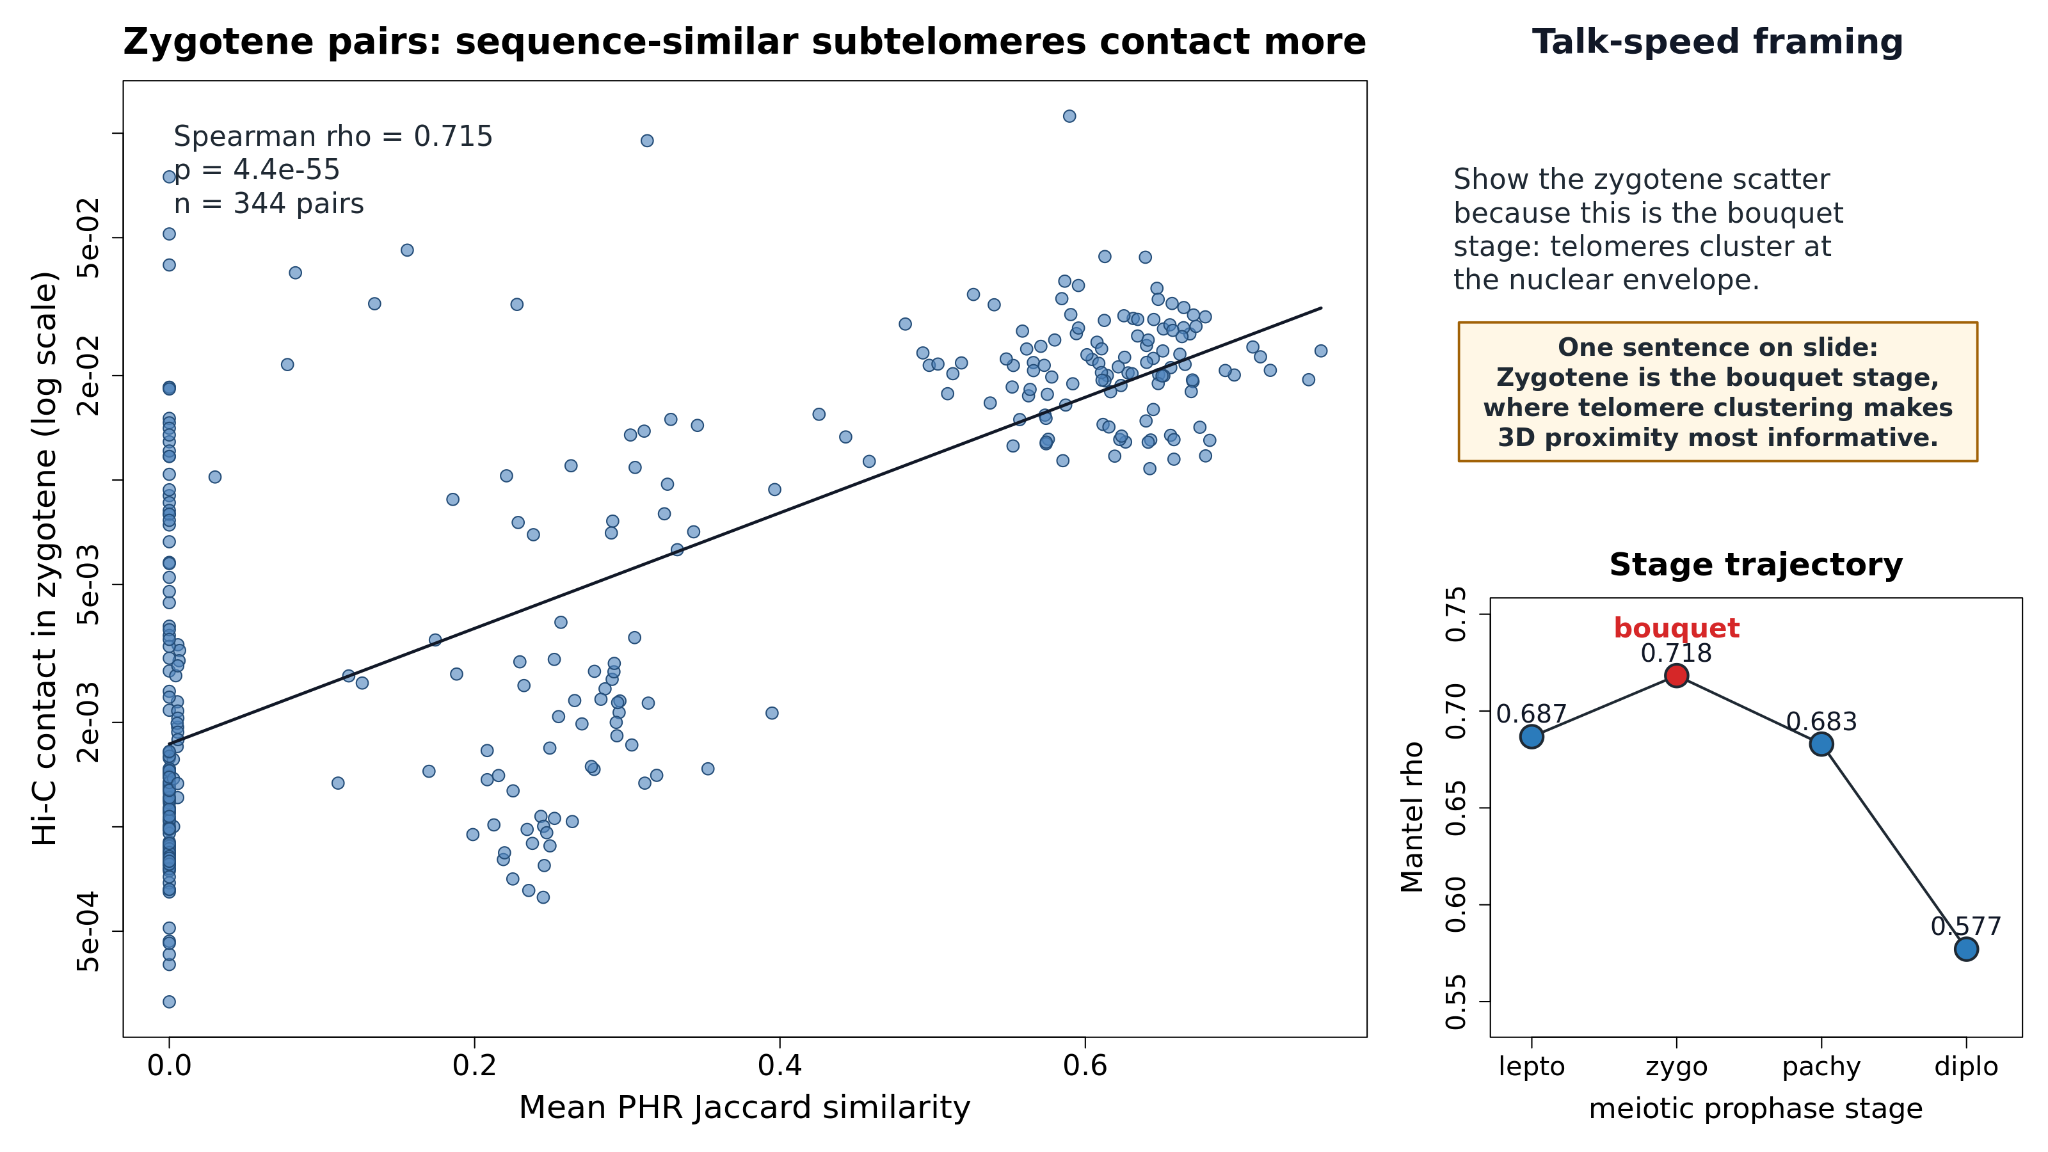
\includegraphics[width=\linewidth]{fig/ExtendedDataFigures/ED_Fig1_mouse_zygotene.png}
  \caption{\textbf{Mouse meiotic Hi-C validates the sequence-to-3D relationship
    at the bouquet stage.}
    Mouse PHRs were established de novo from B6 and CAST T2T assemblies,
    repeating the entire pipeline on a non-human mammal and validating the Hi-C
    approach. Per arm-pair, zygotene Hi-C contact (log scale) rises with mean
    PHR Jaccard similarity (Spearman $\rho = 0.715$, $p = 4.4 \times 10^{-55}$,
    $n = 344$). Inset: Mantel $\rho$ between the $27 \times 27$ arm-level
    Jaccard-distance matrix and Zuo et al.\ (2021) Hi-C contact across meiotic
    prophase stages peaks at the zygotene bouquet (lepto 0.687, zygo 0.718,
    pachy 0.683, diplo 0.577; all $p < 1 \times 10^{-4}$), the only direct
    bouquet-stage 3D measurement in any organism.}
  \label{fig:ed1}
\end{figure}

\end{document}
